\documentclass[8pt]{beamer}

\newif\ifplacelogo % create a new conditional
\placelogotrue % set it to true

\usetheme{Warsaw}
\usecolortheme{rose}
\usepackage{multicol}
\usepackage{epstopdf}
\usepackage[italic]{hepnames}
\usepackage{tikz}
\usepackage{listings}
\usepackage{times}
\usepackage{amsmath}
\usepackage{verbatim}
\usepackage{hyperref}
\usepackage{bbding}
\lstset{breakatwhitespace,
language=C++,
columns=fullflexible,
keepspaces,
breaklines,
tabsize=3, 
showstringspaces=false,
extendedchars=true}

% TikZ includes!!!
\usepackage{tikz}
\usetikzlibrary{backgrounds}
\usetikzlibrary{calc}
\tikzstyle{every picture}+=[remember picture]
\input{/home/oviazlo/Desktop/beamerPresentations/myReports/latexHelpScripts/tikzGrid.tex}


\begin{document}

% custom colors
\definecolor{olive}{rgb}{0.3, 0.4, .1}
\definecolor{fore}{RGB}{249,242,215}
\definecolor{back}{RGB}{51,51,51}
\definecolor{title}{RGB}{255,0,90}
\definecolor{dgreen}{rgb}{0.,0.6,0.}
\definecolor{gold}{rgb}{1.,0.84,0.}
\definecolor{JungleGreen}{cmyk}{0.99,0,0.52,0}
\definecolor{BlueGreen}{cmyk}{0.85,0,0.33,0}
\definecolor{RawSienna}{cmyk}{0,0.72,1,0.45}
\definecolor{Magenta}{cmyk}{0,1,0,0}

\definecolor{PixelColor}{RGB}{207,232,139}
\definecolor{SCTColor}{RGB}{167,166,255}
\definecolor{TRTColor}{RGB}{250,224,140}
\definecolor{grayColor}{RGB}{153,153,153}

\newcommand{\yRefPosOne}{0.0}
\newcommand{\xRefPosOne}{0.0}
\newcommand{\yRefPosTwo}{0.0}
\newcommand{\xRefPosTwo}{0.0}
\newcommand{\yRefIncrementOne}{0.0}
\newcommand{\xRefIncrementOne}{0.0}
\newcommand{\yRefIncrementTwo}{0.0}
\newcommand{\xRefIncrementTwo}{0.0}

\graphicspath{ {/home/oviazlo/Desktop/beamerPresentations/FCCee/pictures/CEPC_workshop/} }
\DeclareGraphicsExtensions{.eps, .pdf, .png}

\newcommand{\myBox}[2][pink] {
    \noindent\colorbox{#1}{
	\textbf{#2}
    }\par
}

% For nice block (provided by Oleh)
\tikzstyle{mybox} = [draw=red, fill=blue!1, very thick,
    rectangle, rounded corners, inner sep=5pt, inner ysep=9pt]
    
\tikzstyle{PixelBox} = [draw=PixelColor, fill=blue!1, very thick,
    rectangle, rounded corners, inner sep=5pt, inner ysep=9pt]
\tikzstyle{SCTBox} = [draw=SCTColor, fill=blue!1, very thick,
    rectangle, rounded corners, inner sep=5pt, inner ysep=9pt]
\tikzstyle{TRTBox} = [draw=TRTColor, fill=blue!1, very thick,
    rectangle, rounded corners, inner sep=5pt, inner ysep=9pt]

% poster advertisement
\newcommand{\myCenterBox}[2][pink] {
   {\centering
    \noindent\colorbox{#1}{
	\textbf{#2}
    }\par
  }
}

\newcommand{\mySmallCenterBox}[2][pink] {
   {\centering
    \noindent\colorbox{#1}{
	\textbf{{\small #2}}
    }\par
  }
}

\newcommand{\myVerySmallCenterBox}[2][pink] {
   {\centering
    \noindent\colorbox{#1}{
	\textbf{{\scriptsize #2}}
    }\par
  }
}

\newcommand{\backupbegin}{
   \newcounter{finalframe}
   \setcounter{finalframe}{\value{framenumber}}
}
\newcommand{\backupend}{
   \setcounter{framenumber}{\value{finalframe}}
}

\newcommand{\myNode}{\tikz[baseline,inner sep=1pt] \node[anchor=base]}

\definecolor{light-gray}{gray}{0.95}
% poster advertisement


\title[ CLIC-Inspired Detector for FCC-ee \hspace{13.5em}\insertframenumber/
\inserttotalframenumber]{ CLIC-Inspired Detector for FCC-ee }


	\author[Oleksandr Viazlo]{Oleksandr Viazlo \\ 
% 	{\small ???}
	}
	\institute{\small CERN\\} 
	
       
	\date{6 November 2017}

% 	\logo{ \ifplacelogo \includegraphics[height=1.8cm]{./ID_week2/lund_uni-logo_s.pdf} \hspace{0.4cm} \fi}

	
   	\frame{\titlepage}

   	

\placelogofalse

%*****************************************************************************
\begin{frame}{\large \large Introduction}

\renewcommand{\yRefPosOne}{0}
\renewcommand{\xRefPosOne}{5.3}
\renewcommand{\xRefIncrementOne}{5.5}

\begin{tikzpicture}[overlay]


 \node[inner sep=0pt] (tmp) at (\xRefPosOne-2.35,\yRefPosOne-2.3)
    {\includegraphics[width=7.8cm]{FCCee_lumi_vs_others_v2.png}};


\node [Box] at (\xRefPosOne-0.5,\yRefPosOne+2.1) (box){%
\begin{minipage}{1.1\textwidth}

 \begin{itemize}
  \item FCC-ee is a high-luminosity, high-precision $e^+e^-$ circular collider with four operational energy regimes: Z, WW, HZ, tt. \\[0.1cm]
  \item Fixed 100 MW Synchrotron Radiation (SR) at all energies $\to$ \\
  Larger beam currents possible at lower energies\\[0.1cm]
  \item High statistical accuracies $\to$ Small experimental uncertainties are needed $\to$ \\
  Demands state-of-the-art performance for all detector subsystems \\[0.1cm]
  \item This presentation will cover one of the proposed detector designs for FCC-ee which is based on the detector proposal for CLIC\\[0.05cm]
  
 \end{itemize}
\end{minipage}
};
 
\node [Box] at (\xRefPosOne+7,\yRefPosOne-0.9) (box){%
\begin{minipage}{\textwidth}
{\small
  \begin{tabular}{c|cc}
	  \hline

	       &  Beam Energy & Luminosity  \\
	       &  [GeV] & [10$^{34}$ cm$^{-2}$s$^{-1}$] \\
	  \hline
	  Z  & 45.6 & 230 \\
	  WW & 80 & 32 \\
	  HZ & 120 & 7.8 \\
	  tt & 182.5 & 1.5 \\
	  


	  
% 	       &  Beam Energy & Bunch spacing \\
% 	       & [GeV] & [ns] \\
% 	  \hline
% 	  Z & 45.6  & 20  \\
% 	  WW & 80  & 166  \\
% 	  HZ & 120  & 846  \\
% 	  tt & 182.5 & 8533  \\
	  \hline
	\end{tabular}
}
\end{minipage}
};

\node [Box] at (\xRefPosOne+7,\yRefPosOne-3.1) (box){%
\begin{minipage}{\textwidth}
{\small
  \begin{tabular}{c|cc}
	  \hline
	  

	  	       &  Bunch intensity & Bunch spacing  \\
	       &  [10$^{11}$] & [ns] \\
	  \hline
	  Z  &   1.7 & 20 \\
	  WW & 1.5 & 166 \\
	  HZ & 1.5 & 846 \\
	  tt & 2.8 & 8533 \\
	  
% 	       &  Bunch intensity & Luminosity  \\
% 	       &  [10$^{11}$] & [10$^{34}$ cm$^{-2}$s$^{-1}$] \\
% 	  \hline
% 	  Z  & 1.7 & 230 \\
% 	  WW & 1.5 & 32 \\
% 	  HZ & 1.5 & 7.8 \\
% 	  tt & 2.8 & 1.5 \\
	  \hline
	\end{tabular}
}
\end{minipage}
};


\end{tikzpicture}
\end{frame}
%*****************************************************************************

%*****************************************************************************
% \bgroup
% \setbeamercolor{background canvas}{bg=white}
\begin{frame}{}

    \begin{tikzpicture}[overlay]

    %% HELPER draw advanced helping grid with axises:
%     \draw (0,-5) to[grid with coordinates] (11,3);

    \node[right] (textNode) at (4,0) {
      { \large \bf Detector Design }
    };
    

    \end{tikzpicture}

\end{frame}
% \egroup
%*****************************************************************************

% %*****************************************************************************
% \begin{frame}{\large \large Detector constrains from the machine design}
%  \begin{tikzpicture}[overlay]
%  \node [Box] at (\xRefPosOne+3.5,\yRefPosOne) (box){%
%     \begin{minipage}{0.5\textwidth}
% 
%   \begin{itemize}
%    \item MDI region - what is inside
%    \item shileding from the beam induced backgrounds
%    \item Final focus quadrupole magnet at 2.2m (inside the detector) 
%    $\to$ compensating solenoid to negate effect of detector magnetic field which blow-up emmitance  
%    $\to$ constrains on dfetector magnetic field (not more than 2T)
%   \end{itemize}
% 
%     \end{minipage}
% };
% 
% \end{tikzpicture}
%  
% \end{frame}
% %*****************************************************************************

%*****************************************************************************
\begin{frame}{\large \large Detector Constraints from the Machine Design}
\renewcommand{\yRefPosOne}{0}
\renewcommand{\xRefPosOne}{5.3}
\renewcommand{\xRefIncrementOne}{5.5}

 \begin{tikzpicture}[overlay]
 
  \node[inner sep=0pt] (tmp) at (\xRefPosOne,\yRefPosOne-2.56)
    {\includegraphics[width=10.8cm]{compensatingAndShieldingSolenoids.png}};

 
 \node [Box] at (\xRefPosOne,\yRefPosOne+1.5) (box){%
    \begin{minipage}{\textwidth}

  \begin{itemize}
   \item In order to maximize luminosity final focusing quadrupole chosen to be at 2.2m from IP - {\bf inside the detector}
%    (together with a shielding solenoid)
%    \item To protect the beam from the detector magnetic field an additional compensating solenoid is needed
   \item Compensating solenoid to prevent emittance blow-up from detector magnetic field 
   due to non-zero crossing angle is even closer to the IP
   \item Constrains {\bf the maximum possible detector magnetic field to 2T} \\(while the CLIC proposal assumes 4T magnetic field)
  \end{itemize}

    \end{minipage}
};

\end{tikzpicture}
 
\end{frame}
%*****************************************************************************

%*****************************************************************************
\begin{frame}{\large \large Machine Detector Interface Region}
\renewcommand{\yRefPosOne}{0}
\renewcommand{\xRefPosOne}{5.3}
\renewcommand{\xRefIncrementOne}{2}

 \begin{tikzpicture}[overlay]
 
  \node[inner sep=0pt] (tmp) at (\xRefPosOne+\xRefIncrementOne-1,\yRefPosOne-2)
    {\includegraphics[width=7.8cm]{IR_with_VertexD_MSullivan_v2.png}};

  \node[inner sep=0pt] (tmp) at (\xRefPosOne-6+\xRefIncrementOne,\yRefPosOne-2)
    {\includegraphics[width=1.5cm]{MDI_region_legend_v2.png}};
 
 \node [Box] at (\xRefPosOne,\yRefPosOne+2) (box){%
    \begin{minipage}{\textwidth}

  \begin{itemize}
   \item Central detector has to be fitted within $\pm$150mrad $\to$ constrains forward region \\[0.1cm]
%    \item Small beampipe radius - allows placing innermost pixel layer at 17mm
   \item Luminosity monitor (LumiCal) is inside MDI region
   \item Additional tantalum shielding is foreseen to suppress synchrotron radiation background in the 
   innermost layers of the detector (see picture)
   
  \end{itemize}
\end{minipage}
};

\end{tikzpicture}
 
\end{frame}
%*****************************************************************************



%*****************************************************************************
\begin{frame}{\large \large Detector for FCC-ee}

\renewcommand{\yRefPosOne}{0}
\renewcommand{\xRefPosOne}{5.3}
\renewcommand{\xRefIncrementOne}{5.5}
\begin{tikzpicture}[overlay]

 \node[inner sep=0pt] (tmp) at (\xRefPosOne-2.15,\yRefPosOne-0.56)
    {\includegraphics[width=7.8cm]{FCCeePictsFromKonrad/CLIC_FCC_Top_QuarterView_withLabes.png}};

    \draw[black, thick, ->] (-0.8,-4.76)--(-0.8,3.7) node[pos=0.95, right]{\small R [m]};
    \draw[black, thick, ->] (-0.8,-4.76)--(6.5,-4.76) node[pos=0.95, below]{\tiny Z [m]};
    
  \node[inner sep=0pt] (tmp) at (\xRefPosOne-3.05,\yRefPosOne-4.9)
    {2.3};   
  \node[inner sep=0pt] (tmp) at (\xRefPosOne-1.14,\yRefPosOne-4.9)
    {3.7};  
    
    
\node [Box] at (\xRefPosOne+3.5,\yRefPosOne) (box){%
    \begin{minipage}{0.5\textwidth}

  \begin{itemize}
   \item Full silicon VTX and Tracker:  
   \begin{itemize}
    \item $\geqslant$12 hits per track 
    \item r$_{inner} = 17$mm, r$_{outer} = 2.1$m \\
         {\color{gray} r$_{inner} = 31$mm, r$_{outer} = 1.5$m - CLIC}\\[0.3cm]
    
   \end{itemize}

   
%    \\ \hspace{0.1cm}  r$_{inner} = 17$mm, r$_{outer} = 2.1$m \\ \hspace{0.1cm} $\geqslant$12 hits per track
   \item W-Si ECAL 
   \begin{itemize}
    \item 40 layers, 22 X$_0$ \\[0.3cm]
   \end{itemize}
   \item Fe-Scint HCAL
   \begin{itemize}
    \item 44 layers, 5.5 $\lambda_I$ \\[0.3cm]
   \end{itemize}
   \item 2 Tesla magnetic field, \\
   Coil is outside of the calorimeter\\[0.3cm]
   \item Steel return yoke with 6 RPC muon chambers (1.5m thickness)\\[0.3cm]
   \item MDI (forward region): $<$ 150 mrad, \\
   accommodates LumiCal\\[0.3cm]
  \end{itemize}

    \end{minipage}
};


\node [PixelBox] at (\xRefPosOne+3.7,\yRefPosOne-4) (box){%
  \begin{minipage}{0.43\textwidth}
    Detector design inspired by detectors for CLIC and ILC and optimized for FCC-ee conditions
  \end{minipage}
};

%% HELPER draw advanced helping grid with axises:
% \draw(-0.5,-4) to[grid with coordinates] (11.5,4);
\end{tikzpicture}

 
\end{frame}
%*****************************************************************************


%*****************************************************************************
\begin{frame}{\large \large Software}

\renewcommand{\yRefPosOne}{0}
\renewcommand{\xRefPosOne}{5.3}
\renewcommand{\xRefIncrementOne}{5.5}
\begin{tikzpicture}[overlay]

%  \node[inner sep=0pt] (tmp) at (\xRefPosOne-2.15,\yRefPosOne-0.56)
%     {\includegraphics[width=7.8cm]{FCCeePictsFromKonrad/CLIC_FCC_Top_QuarterView_withLabes.png}};

    
\node [Box] at (\xRefPosOne,\yRefPosOne) (box){%
    \begin{minipage}{\textwidth}

  \begin{itemize}
   \item Dedicated software for FCC-ee is under development.
   \item For performance study of the CLIC-inspired detector for FCC-ee 
	 one can benefit from the fully functional and tested \href{https://github.com/iLCSoft}{\color{blue} iLCSoft} software used by the CLIC and ILC community. \\[0.4cm]
   
   \item Detector geometry description and event simulation: \href{https://github.com/AIDASoft/DD4hep}{\color{blue} DD4hep}
   \item Event Reconstruction: \href{https://github.com/iLCSoft/Marlin}{\color{blue} Marlin}\\[0.4cm]
   
   \item Track Pattern recognition: TruthTracking or ConformalTracking
   \item Particle Flow Reconstruction: \href{https://github.com/PandoraPFA}{\color{blue} PandoraPFA} \\[0.6cm]
   
   \item Detector model: \\
   \href{https://github.com/iLCSoft/lcgeo/tree/master/FCCee/compact/FCCee_o1_v01}{\color{blue}  https://github.com/iLCSoft/lcgeo/tree/master/FCCee/compact/FCCee$\_$o1$\_$v01}
  \end{itemize}

    \end{minipage}
};



%% HELPER draw advanced helping grid with axises:
% \draw(-0.5,-4) to[grid with coordinates] (11.5,4);
\end{tikzpicture}

 
\end{frame}
%*****************************************************************************

%*****************************************************************************
\begin{frame}{\large \large VTX and Tracker Layout}
 
\renewcommand{\yRefPosOne}{0}
\renewcommand{\xRefPosOne}{5.3}
\renewcommand{\xRefIncrementOne}{5.5}
\begin{tikzpicture}[overlay]

%  \node[inner sep=0pt] (tmp) at (\xRefPosOne,\yRefPosOne-1.9)
%     {\includegraphics[width=12cm]{CLIC_vs_FCCee_trackingSystem.png}};

    
\node [Box] at (\xRefPosOne,\yRefPosOne+2) (box){%
    \begin{minipage}{1.1\textwidth}

      \begin{itemize}
       \item Tracking system consists of Vertex detector(VTX), Inner and Outer Trackers (IT and OT)
       \item VTX detector - 3 pixel double layers in barrel and endcap
       \item Inner and Outer Trackers - 3 barrel layers each and 4-7 disks
       \item Single-point resolution (sigma): VTX - 3$\times$3 $\mu$m; IT - 7$\times$300$\mu$m; OT - 7$\times$3000$\mu$m
       \item More than 12 hits per track over theta range 8.6$^{\circ}$ - 171.4$^{\circ}$
       \item Material budget: 0.2$\%$X0 per VTX layer - has to be revised due to the need for cooling
%        (small affect on tracking is expected)
      \end{itemize}

    \end{minipage}
};
% \node[fancytitle, right=15pt] at (box.north west) {Transition Radiation Tracker};

 \node[inner sep=0pt] (tmp) at (\xRefPosOne,\yRefPosOne-2.2)
%     {\includegraphics[width=12cm]{CLIC_vs_FCCee_trackingSystem.png}};
  {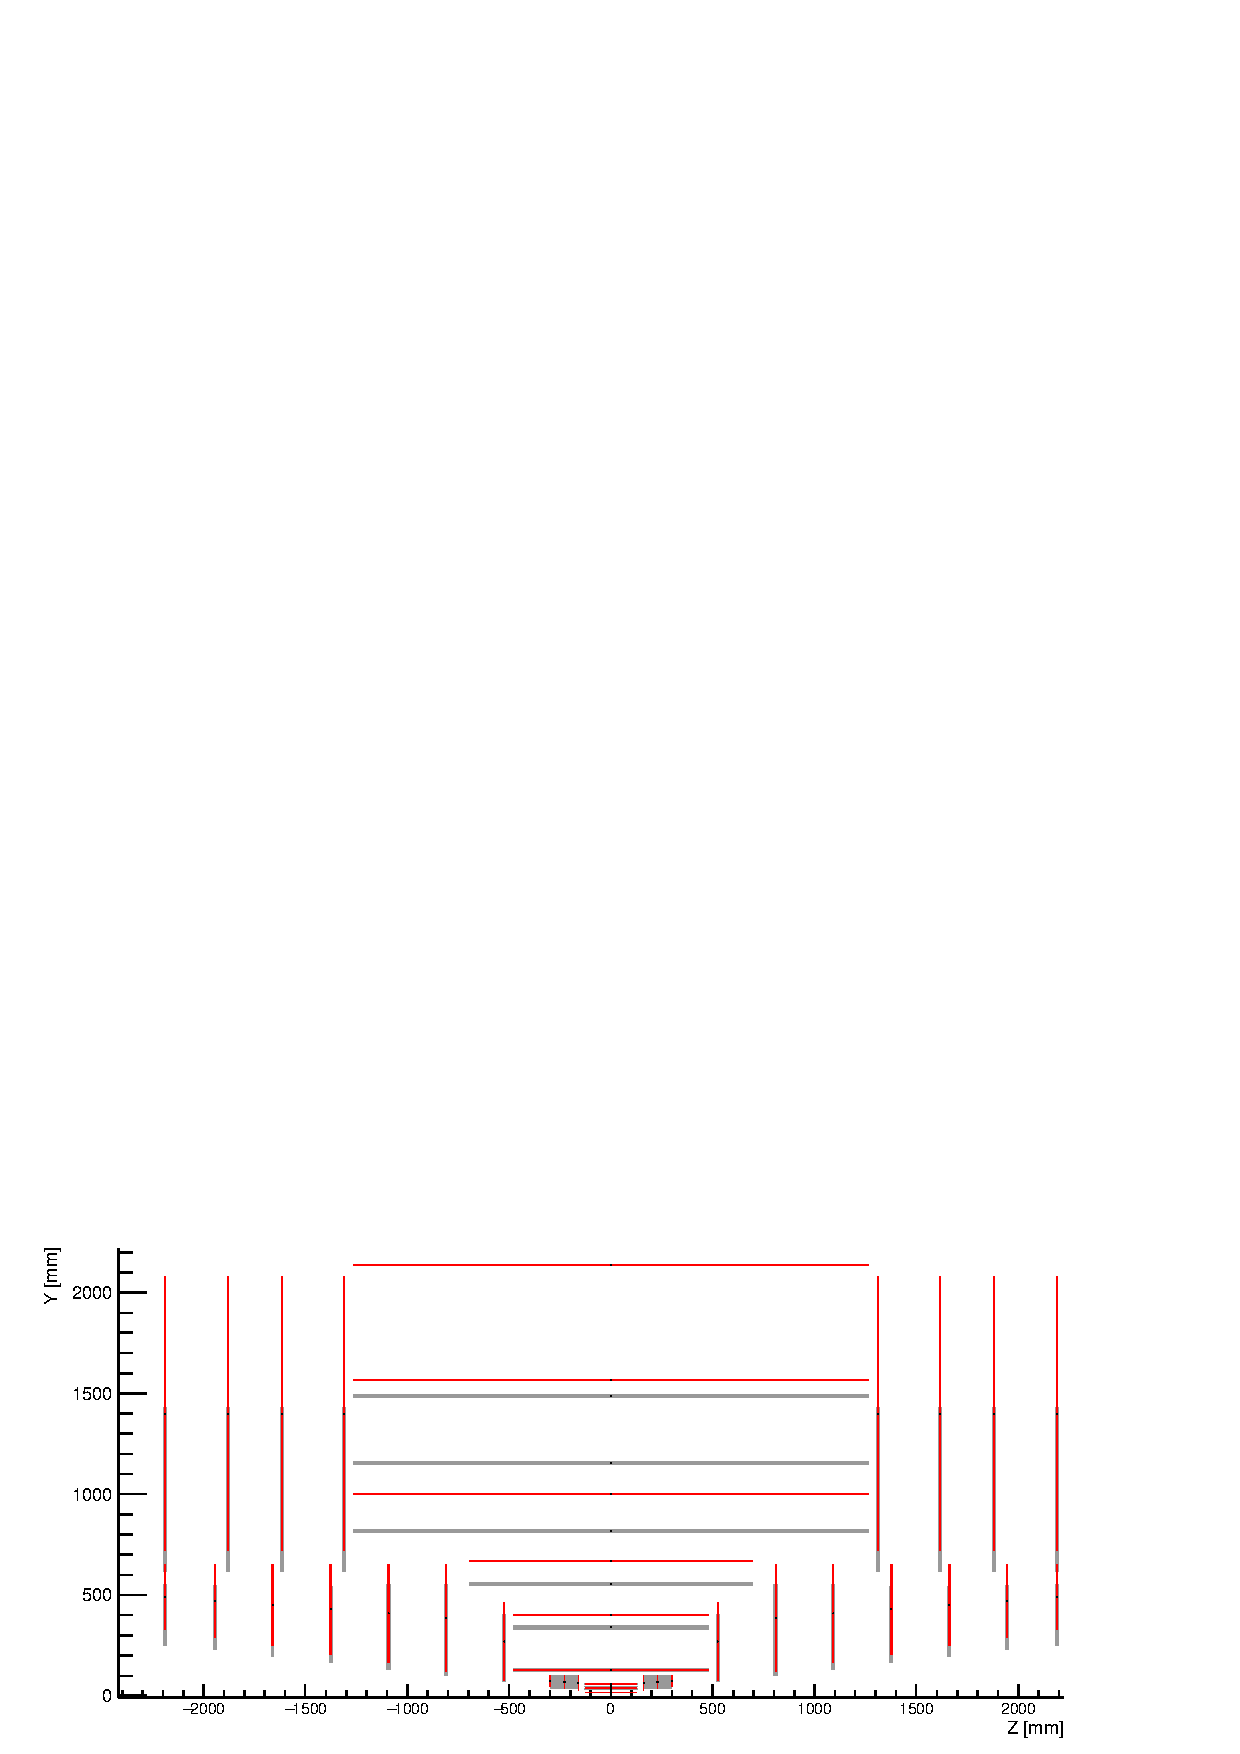
\includegraphics[width=12cm]{../geometryComparison_v3.pdf}};


\node [Box] at (\xRefPosOne,\yRefPosOne+0.4) (box){%
\myCenterBox{Comparison of the CLIC and FCC-ee tracking system}
};
    
\node [Box] at (\xRefPosOne+5.35,\yRefPosOne-1.8) (box){%
\myVerySmallCenterBox[grayColor]{CLIC}
};
    
\node [Box] at (\xRefPosOne+5.35,\yRefPosOne-2.5) (box){%
\myVerySmallCenterBox[red]{FCC-ee}
};
    
%% HELPER draw advanced helping grid with axises:
% \draw(-0.5,-4) to[grid with coordinates] (11.5,4);
\end{tikzpicture}

  
\end{frame}
%*****************************************************************************

%*****************************************************************************
% \bgroup
% \setbeamercolor{background canvas}{bg=white}
\begin{frame}{}

    \begin{tikzpicture}[overlay]

    %% HELPER draw advanced helping grid with axises:
%     \draw (0,-5) to[grid with coordinates] (11,3);

    \node[right] (textNode) at (3.5,0) {
      { \large \bf FCC-ee backgrounds }
    };
    

    \end{tikzpicture}

\end{frame}
% \egroup
%*****************************************************************************

%*****************************************************************************
\begin{frame}{\large \large Background estimate}
% TODO change legend for electron plot. ``Nominal'' -> ``Default Pandora''

\renewcommand{\yRefPosOne}{0}
\renewcommand{\xRefPosOne}{5.3}
\renewcommand{\xRefIncrementOne}{5.5}
\begin{tikzpicture}[overlay]

 \node[inner sep=0pt] (tmp) at (\xRefPosOne+3,\yRefPosOne+1.5)
    {\includegraphics[width=6cm]{bkg_FCCee_91GeV.png}};
    
 \node[inner sep=0pt] (tmp) at (\xRefPosOne+3,\yRefPosOne-2.7)
    {\includegraphics[width=6cm]{bkg_FCCee_350GeV.png}};
    
 \node[inner sep=0pt] (tmp) at (\xRefPosOne+4.2,\yRefPosOne+2.7)
    {\tiny WORK IN PROGRESS};
    
 \node[inner sep=0pt] (tmp) at (\xRefPosOne+4.2,\yRefPosOne-1.5)
    {\tiny WORK IN PROGRESS};
    
\node [Box] at (\xRefPosOne-3.4,\yRefPosOne+2) (box){%
    \begin{minipage}{0.5\textwidth}

  \begin{itemize}
  \item $\gamma\gamma \to e^+e^-$\\[0.1cm]
  \item $\gamma\gamma \to$ hadrons \\[0.1cm]
  \item Synchrotron radiation\\[0.1cm]
 \end{itemize}
    \end{minipage}
};

\node [Box] at (\xRefPosOne-4.5,\yRefPosOne+3) (box){%
\myCenterBox{FCC-ee Backgrounds}
}; 

\node [Box] at (\xRefPosOne-3.4,\yRefPosOne-2) (box){%
\begin{minipage}{0.5\textwidth}
  \begin{itemize}
  \item Full simulation (GuineaPig, GEANT/DD4hep)\\[0.2cm]
  \item Detector assumptions:
  \begin{itemize}
    \item pixel silicon detector, 25$\times$25$\mu$m$^2$
    \item strip detector, 1$\times$0.05 mm$^2$
    \item Cluster multiplicity = 5 for pixels and = 2.5 for strips\\[0.2cm]
  \end{itemize}
  \item Safety factor: 5\\[0.2cm]
  \item Occupancy is estimated in the VTX and Tracker detectors

  \end{itemize}
\end{minipage}
};


\node [Box] at (\xRefPosOne-4,\yRefPosOne+0.5) (box){%
\myCenterBox{Background Estimation}
}; 

% \node [Box] at (\xRefPosOne-3.4,\yRefPosOne-3.3) (box){%
% \begin{minipage}{0.5\textwidth}
%   \begin{itemize}
%    \item $\approx$ 5$\cdot$10$^{-4}$ per BX {\tiny (both for 91 and 350 GeV)}
%    \item 1$\%$ occupancy $\to$ 0.4 $\mu s$ read-out time
%   \end{itemize}
% \end{minipage}
% };
% 
% \node [Box] at (\xRefPosOne-4,\yRefPosOne-2.5) (box){%
% \myCenterBox{Detector occupancy}
% }; 



%% HELPER draw advanced helping grid with axises:
% \draw(-0.5,-4) to[grid with coordinates] (11.5,4);
\end{tikzpicture}
 
\end{frame}
%*****************************************************************************




%*****************************************************************************
\begin{frame}{\large \large Background Estimate: $\gamma\gamma \to e^+e^-$}
% TODO change legend for electron plot. ``Nominal'' -> ``Default Pandora''

\renewcommand{\yRefPosOne}{-0.5}
\renewcommand{\xRefPosOne}{5.3}
\renewcommand{\xRefIncrementOne}{5.5}
\begin{tikzpicture}[overlay]

 \node[inner sep=0pt] (tmp) at (\xRefPosOne-3,\yRefPosOne+1.2)
    {\includegraphics[width=5.5cm]{Yorgos/bkg_vtx_91GeV.pdf}};
    
 \node[inner sep=0pt] (tmp) at (\xRefPosOne+3,\yRefPosOne+1.25)
    {\includegraphics[width=5.2cm]{Yorgos/bkg_vtx_350GeV.png}};
    
 \node[inner sep=0pt] (tmp) at (\xRefPosOne-1.6,\yRefPosOne+0.1)
    {\tiny WORK IN PROGRESS};
 \node[inner sep=0pt] (tmp) at (\xRefPosOne+4.5,\yRefPosOne-0.1)
    {\tiny WORK IN PROGRESS};
    
\node [Box] at (\xRefPosOne-4.01,\yRefPosOne+3.1) (box){%
\myCenterBox{\small 91.2 GeV}
}; 
\node [Box] at (\xRefPosOne-3.9,\yRefPosOne+2.75) (box){%
\myCenterBox{\small VTX Barrel}
}; 

\node [Box] at (\xRefPosOne+3.1,\yRefPosOne+3.33) (box){%
\myCenterBox{\small 350 GeV, VTX Barrel}
}; 



\node [Box] at (\xRefPosOne+3,\yRefPosOne-2.8) (box){%
\begin{minipage}{0.6\textwidth}
  \begin{itemize}
   \item Maximum 0.05$\%$ per BX both for 91.2 and 350 GeV cases from $\gamma\gamma \to e^+e^-$ background
%    \item 1$\%$ occupancy $\to$ 0.4 $\mu s$ read-out time\\[0.25cm]
   \item Need $\approx$0.4 $\mu s$ read-out time at 91.2 GeV, to limit the occupancy to 1$\%$
   \item Study at 365 GeV center-of-mass energy is ongoing. 
	Preliminary results are of similar size as for 350 GeV case
  \end{itemize}
\end{minipage}
};

% \node [Box] at (\xRefPosOne+3,\yRefPosOne-2.2) (box){%
% \myCenterBox{Detector occupancy}
% }; 

\node [Box] at (\xRefPosOne-3,\yRefPosOne-2.99) (box){%
\begin{minipage}{0.5\textwidth}
  \begin{tabular}{c|cc}
	  \hline
	    E$_{CM}$   & 91.2 GeV & 350 GeV \\
	  \hline
	  VTX Barrel & 0.05 $\%$ & 0.05 $\%$ \\
	  VTX Endcap & 0.02 $\%$ & 0.03 $\%$ \\
	  Tracker B. & 0.002 $\%$ & 0.0025 $\%$ \\
	  Tracker E. & 0.014 $\%$ & 0.0075 $\%$ \\
	  \hline
	\end{tabular}

\end{minipage}
};

\node [Box] at (\xRefPosOne-3,\yRefPosOne-1.8) (box){%
\myCenterBox{\small Maximum occupancy per BX}
}; 

%  \node[inner sep=0pt] (tmp) at (\xRefPosOne+3,\yRefPosOne-3.13)
%     {\includegraphics[width=4.5cm]{Yorgos/hadrons.png}};
% 
%     \node[inner sep=0pt] (tmp) at (\xRefPosOne+2.3,\yRefPosOne-4)
%   {\tiny WORK IN PROGRESS};
%     
% \node [Box] at (\xRefPosOne+3,\yRefPosOne-1.3) (box){%
% \myCenterBox{\small Estimate of $\gamma\gamma \to$ hadrons bkg. }
% }; 
% \node [Box] at (\xRefPosOne+3,\yRefPosOne-1.6) (box){%
% \myCenterBox{\tiny Hits per BX per subdetector}
% }; 




%% HELPER draw advanced helping grid with axises:
% \draw(-0.5,-4) to[grid with coordinates] (11.5,4);
\end{tikzpicture}
 
\end{frame}
%*****************************************************************************

%*****************************************************************************
\begin{frame}{\large \large Background Estimate}
% TODO change legend for electron plot. ``Nominal'' -> ``Default Pandora''

\renewcommand{\yRefPosOne}{4}
\renewcommand{\xRefPosOne}{-0.7}
\renewcommand{\xRefIncrementOne}{-0.5}
\begin{tikzpicture}[overlay]


\node [Box] at (\xRefPosOne+9,\yRefPosOne-1.3) (box){%
\myCenterBox{\small Synchrotron radiation}
}; 

\node [Box] at (\xRefPosOne+9,\yRefPosOne-2.8) (box){%
\begin{minipage}{0.5\textwidth}
  \begin{itemize}
   \item Study is ongoing
   \item Preliminary results show negligable effect for 91.2 GeV case and comparable effect to $\gamma\gamma \to e^+e^-$ for 350/365 GeV cases
  \end{itemize}
\end{minipage}
};

 \node[inner sep=0pt] (tmp) at (\xRefPosOne+9,\yRefPosOne-6)
    {\includegraphics[width=5.5cm]{SR_nicePict.png}};

 \node[inner sep=0pt] (tmp) at (\xRefPosOne+3,\yRefPosOne-3.53)
    {\includegraphics[width=4.5cm]{Yorgos/hadrons.png}};

    \node[inner sep=0pt] (tmp) at (\xRefPosOne+2.3,\yRefPosOne-4.4)
  {\tiny WORK IN PROGRESS};
    
\node [Box] at (\xRefPosOne+3,\yRefPosOne-1.3) (box){%
\myCenterBox{\small Estimate of $\gamma\gamma \to$ hadrons bkg. }
}; 
\node [Box] at (\xRefPosOne+3,\yRefPosOne-2) (box){%
\myCenterBox{\tiny Hits per BX per subdetector at 91.2 GeV}
}; 

\node [Box] at (\xRefPosOne+3,\yRefPosOne-6.1) (box){%
\begin{minipage}{0.5\textwidth}
  \begin{itemize}
   \item Size of $\gamma\gamma \to$ hadrons background is \\ 
   {\bf 2 orders of magnitude lower} than from $\gamma\gamma \to e^+e^-$ $\to$ negligable effect
  \end{itemize}
\end{minipage}
};



%% HELPER draw advanced helping grid with axises:
% \draw(-0.5,-4) to[grid with coordinates] (11.5,4);
\end{tikzpicture}
 
\end{frame}
%*****************************************************************************

%*****************************************************************************
% \bgroup
% \setbeamercolor{background canvas}{bg=white}
\begin{frame}{}

    \begin{tikzpicture}[overlay]

    %% HELPER draw advanced helping grid with axises:
%     \draw (0,-5) to[grid with coordinates] (11,3);

    \node[right] (textNode) at (2,0) {
      { \large \bf Tracking and Calorimetry Performance }
    };
    

    \end{tikzpicture}

\end{frame}
% \egroup
%*****************************************************************************


%*****************************************************************************
\begin{frame}{\large \large Conformal Tracking}
 
 
 \renewcommand{\yRefPosOne}{0}
\renewcommand{\xRefPosOne}{5.3}
\renewcommand{\xRefIncrementOne}{5.5}
\begin{tikzpicture}[overlay]

      
\node [Box] at (\xRefPosOne+3.5,\yRefPosOne+1.5) (box){%
  \begin{minipage}{0.6\textwidth}
 \begin{itemize}
  \item Track fitting is done in the conformal space:\\[1.4cm]
  \item Cellular automaton is used to perform \\straight line search
    \end{itemize}
  \end{minipage}
};

 \node[inner sep=0pt] (tmp) at (\xRefPosOne+3.5,\yRefPosOne+1.7)
    {\includegraphics[width=5cm]{confCoord.png}};


 \node[inner sep=0pt] (tmp) at (\xRefPosOne-2.7,\yRefPosOne+1)
    {\includegraphics[width=7cm]{conformal_tracking.png}};

    
    
\node [Box] at (\xRefPosOne,\yRefPosOne-3.5) (box){%
    \begin{minipage}{0.99\textwidth}

  \begin{itemize}
  \item Conformal tracking is used as the main track pattern recognition algorithm at CLIC
 \end{itemize}

    \end{minipage}
};

    
    
\node[inner sep=0pt] (tmp) at (\xRefPosOne,\yRefPosOne-4)
  {\myCenterBox[yellow]{\href{https://agenda.linearcollider.org/event/7645/contributions/40123/attachments/32387/49200/Leogrande_LCWS2017.pdf}
  {{\tiny LCWS presentation about CLIC Conformal Tracking performance }}}  };
  
% \draw[thick,red,rotate=45] (5,5) ellipse (10pt and 20pt);
\draw[thick,red,rotate=20] (4.6,0.15) ellipse (0.52cm and 0.13cm);
\node[right] (textNode) at (6.5,-1) {Hits from the Vertex};
\draw[thick,red,->] (4.8,1.9) to [out=0, in=135]  ([xshift=0.0cm]textNode.west);
  
\draw[thick,red] (2.95,1.3) ellipse (0.5cm and 0.5cm);
\node[right] (textNode) at (0.5,-2) {Hits from the Tracker};
\draw[thick,red,->] (2.45,1.38) to [out=180, in=135]  ([xshift=0.0cm]textNode.west);
  
%% HELPER draw advanced helping grid with axises:
% \draw(-0.5,-4) to[grid with coordinates] (11.5,4);
  
\end{tikzpicture}
  
 
\end{frame}
%*****************************************************************************
%*****************************************************************************
\begin{frame}{\large \large Momentum and Transverse Impact Parameter Resolution}

\renewcommand{\yRefPosOne}{0}
\renewcommand{\xRefPosOne}{5.3}
\renewcommand{\xRefIncrementOne}{5.5}
\begin{tikzpicture}[overlay]

 \node[inner sep=0pt] (tmp) at (\xRefPosOne-3,\yRefPosOne+1)
    {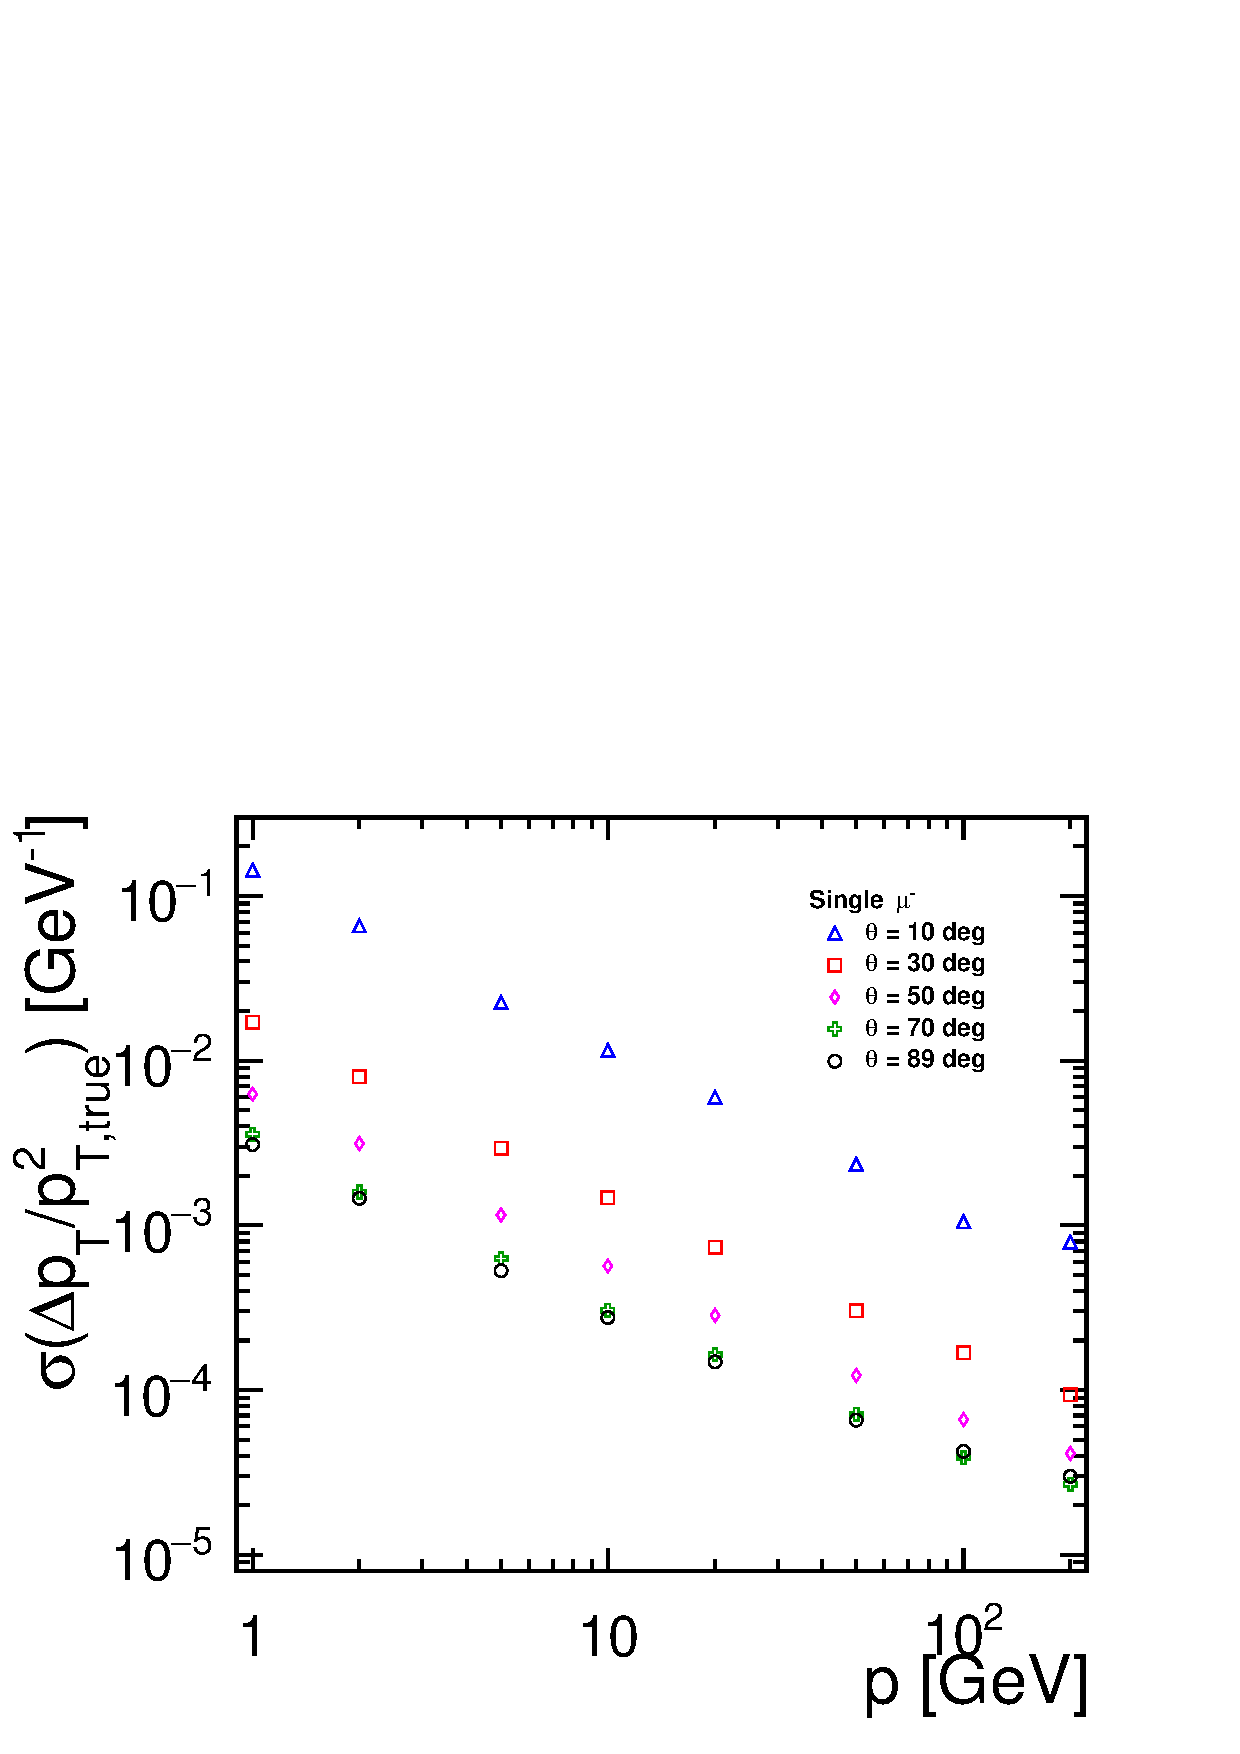
\includegraphics[width=6cm]{MomRes_vs_p.pdf}};

 \node[inner sep=0pt] (tmp) at (\xRefPosOne+3,\yRefPosOne+1)
    {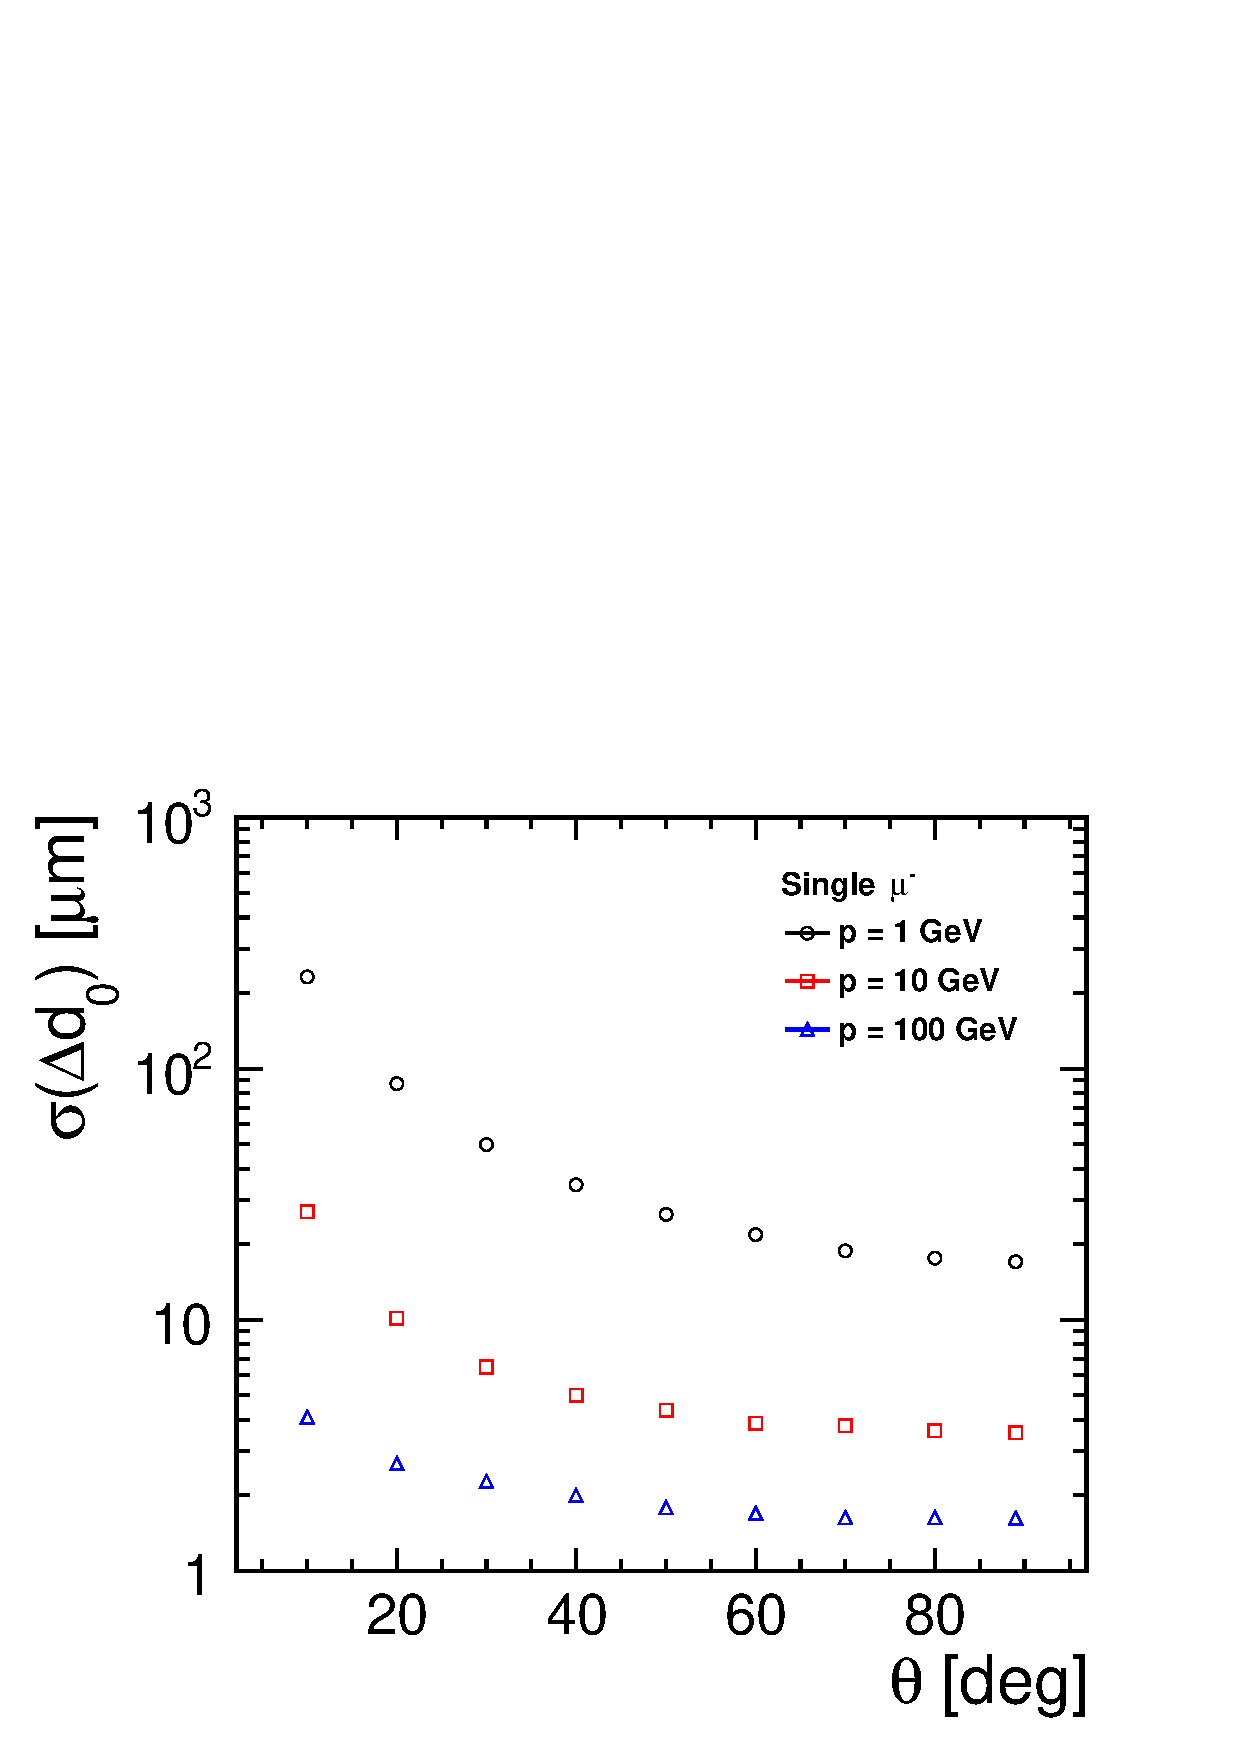
\includegraphics[width=6cm]{d0Resolution.pdf}};
    
 \node[inner sep=0pt] (tmp) at (\xRefPosOne-3.3,\yRefPosOne+2.85)
  {\tiny WORK IN PROGRESS};
 \node[inner sep=0pt] (tmp) at (\xRefPosOne+2.7,\yRefPosOne+2.85)
  {\tiny WORK IN PROGRESS};
    
\node [PixelBox] at (\xRefPosOne-3,\yRefPosOne-2.5) (box){
    \begin{minipage}{0.34\textwidth}
    $\sigma_{\mathrm{p_T}}/ \mathrm{p_T}^2 \simeq$ 4$\cdot$10$^{-5}$ GeV$^{-1}$  \\ at p = 100 GeV at 89$^{\circ}$
    \end{minipage}
};

\node [PixelBox] at (\xRefPosOne+3,\yRefPosOne-2.5) (box){
    \begin{minipage}{0.3\textwidth}
     $\sim$2 $\mu m$ at 100 GeV\\
     $\sim$6 $\mu m$ at 10 GeV\\
     $\sim$12 $\mu m$ at 1 GeV
    \end{minipage}
};

% \node[fancytitle, right=15pt] at (box.north west) {Transition Radiation Tracker};

\node [Box] at (\xRefPosOne,\yRefPosOne-4) (box){%
    \begin{minipage}{0.99\textwidth}

  \begin{itemize}
  \item Detector tracking performance with single muon
  \item Excellent impact parameter resolution, as required for efficient b- and c-tagging
%   \item TODO to highlight numbers for impact parameter resolution
 \end{itemize}

    \end{minipage}
};

%% HELPER draw advanced helping grid with axises:
% \draw(-0.5,-4) to[grid with coordinates] (11.5,4);
\end{tikzpicture}
 
\end{frame}
%*****************************************************************************
%*****************************************************************************
\begin{frame}{\large \large Tracking Efficiency}

\renewcommand{\yRefPosOne}{0}
\renewcommand{\xRefPosOne}{5.3}
\renewcommand{\xRefIncrementOne}{5.5}
\begin{tikzpicture}[overlay]

 \node[inner sep=0pt] (tmp) at (\xRefPosOne-3,\yRefPosOne+1)
    {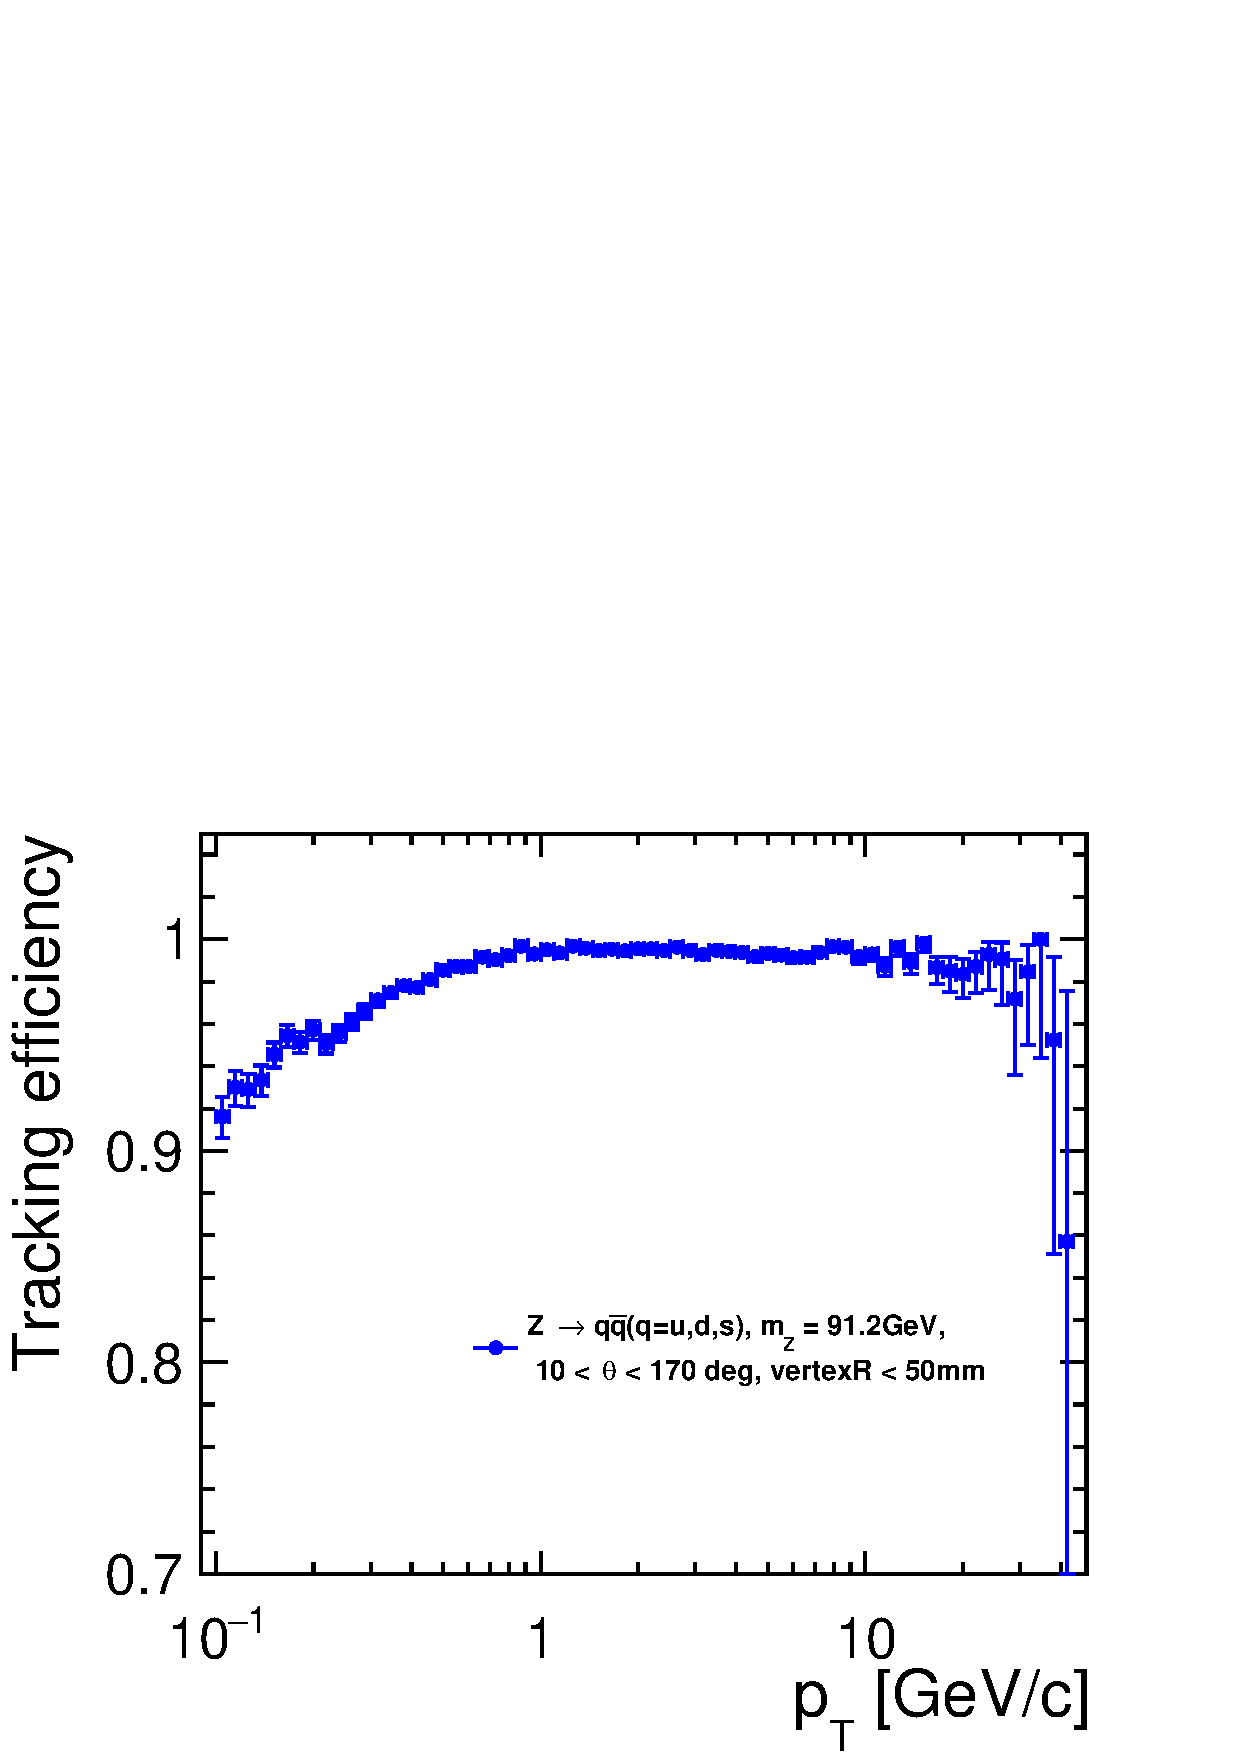
\includegraphics[width=6cm]{c_pt_Zuds91GeV.pdf}};
  \node [Box] at (\xRefPosOne-2.8,\yRefPosOne+3.3) (box){%
    \myCenterBox{\small Z$\to q\bar{q}$ (q=u,d,s), m$_{Z}$ = 91.2 GeV}
  }; 

 \node[inner sep=0pt] (tmp) at (\xRefPosOne+3,\yRefPosOne+1)
    {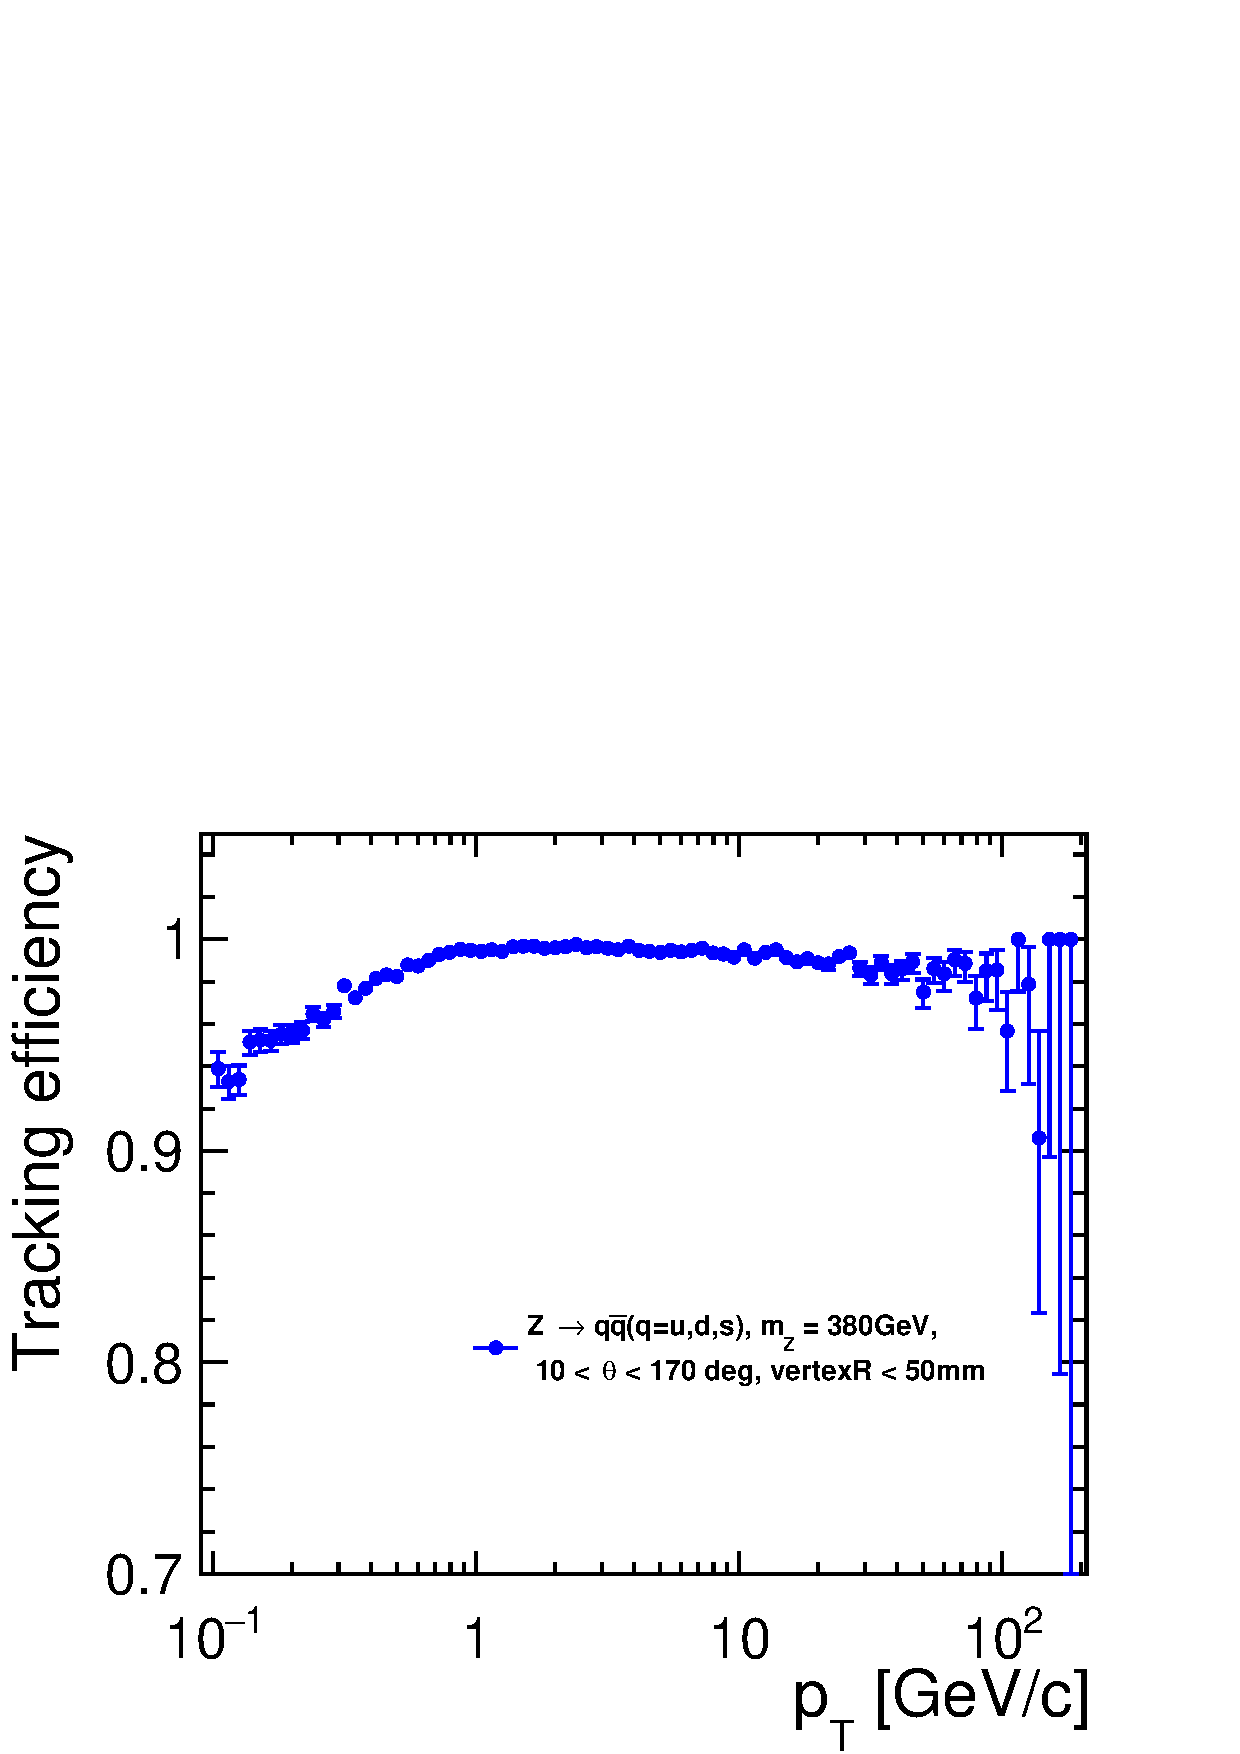
\includegraphics[width=6cm]{c_pt_Zuds380GeV.pdf}};
   \node [Box] at (\xRefPosOne+3.2,\yRefPosOne+3.3) (box){%
    \myCenterBox{\small Z$\to q\bar{q}$ (q=u,d,s), m$_{Z}$ = 380 GeV}
  }; 
  
 \node[inner sep=0pt] (tmp) at (\xRefPosOne-3.3,\yRefPosOne+2.85)
  {\tiny WORK IN PROGRESS};
 \node[inner sep=0pt] (tmp) at (\xRefPosOne+2.7,\yRefPosOne+2.85)
  {\tiny WORK IN PROGRESS};
    
% \node [mybox] at (\xRefPosOne-3,\yRefPosOne-2.5) (box){
%     \begin{minipage}{0.34\textwidth}
% 
%     $\sigma_{\mathrm{p_T}}/ \mathrm{p_T}^2 \simeq$ ?.? $\cdot$ 10$^{-5}$ GeV$^{-1}$  \\ at p = 100 GeV at 89$^{\circ}$
%     
% %       \begin{itemize}
% % 	\item $\sigma_{\mathrm{p_T}}/ \mathrm{p_T}^2 \simeq$ 4.8 $\cdot$ 10$^{-5}$ GeV$^{-1}$ \\at p$_\mathrm{T}$ = 100 GeV at 90$^{\circ}$
% %       \end{itemize}
% 
%     \end{minipage}
% };
% \node[fancytitle, right=15pt] at (box.north west) {Transition Radiation Tracker};


\node [PixelBox] at (\xRefPosOne-3,\yRefPosOne-2.5) (box){%
  \begin{minipage}{0.43\textwidth}
Tracking efficiency = $\dfrac{N^{reconstructed}_{tracks}}{N^{reconstructable}_{particles}}$
  \end{minipage}
};
      
\node [Box] at (\xRefPosOne+3,\yRefPosOne-2.8) (box){%
  \begin{minipage}{0.5\textwidth}
    \begin{itemize}
      \item reconstructable particles:
      \begin{itemize}
%        \item PDG ID = 13 (muon)
       \item N$_{hits} \geqslant$ 4
       \item $|$cos$(\theta)| <$ 0.99
       \item p$_\mathrm{T} \geqslant$ 0.1 GeV/c
%        \item dist from IP < 10 cm
       \item particle track is not a loop \\(does not have two hits on the same layer of the same subdetector)
      \end{itemize}

    \end{itemize}
  \end{minipage}
};

% \node [Box] at (\xRefPosOne,\yRefPosOne-3.2) (box){%
%     \begin{minipage}{0.99\textwidth}
% 
%   \begin{itemize}
%   \item Muon particle gun 
%   \item TODO Define efficiency
%   
%  \end{itemize}
% 
%     \end{minipage}
% };

%% HELPER draw advanced helping grid with axises:
% \draw(-0.5,-4) to[grid with coordinates] (11.5,4);
\end{tikzpicture}
 
\end{frame}
%*****************************************************************************

%*****************************************************************************
\begin{frame}{\large \large Calorimeter}
 
\renewcommand{\yRefPosOne}{0}
\renewcommand{\xRefPosOne}{5.3}
\renewcommand{\xRefIncrementOne}{5.5}
\begin{tikzpicture}[overlay]

%  \node[inner sep=0pt] (tmp) at (\xRefPosOne,\yRefPosOne-1.9)
%     {\includegraphics[width=12cm]{CLIC_vs_FCCee_trackingSystem.png}};

\node [Box] at (\xRefPosOne-3,\yRefPosOne+1.7) (box){%
    \begin{minipage}{0.5\textwidth}
    \begin{itemize}
       \item SiW sampling calorimeter\\[0.1cm]
       \item Cell size: 5x5 mm$^2$\\[0.1cm]
       \item 40 layers, 22 $X_0$\\[0.1cm]
       \item Identical to CLIC ECAL $\to$ to keep good photon energy resolution
    \end{itemize}
    \end{minipage}
};
\node [Box] at (\xRefPosOne-4,\yRefPosOne+3.2) (box){%
\myCenterBox{ECAL}
};

\node [Box] at (\xRefPosOne+3,\yRefPosOne+1.7) (box){%
    \begin{minipage}{0.5\textwidth}
    \begin{itemize}
       \item steel + scintillator sampling calorimeter\\[0.1cm]
       \item Cell size: 3x3 cm$^2$ \\[0.1cm]
       \item 44 layers, 5.5 $\lambda_I$\\[0.1cm]
       \item Depth is inspired by HCAL for ILD detector (optimized for 500 GeV)
    \end{itemize}
    \end{minipage}
};
\node [Box] at (\xRefPosOne+2,\yRefPosOne+3.2) (box){%
\myCenterBox{HCAL}
};
    
\node [Box] at (\xRefPosOne,\yRefPosOne-2) (box){%
    \begin{minipage}{1.1\textwidth}

      \begin{itemize}
%        \item TODO Some detail about ECAL and HCAL dimensions
%        \item TODO Size of read-out pixels, thickness per layer, explain that we want to have as small as possible Moliere radius (for PFA)\\[0.5cm]
       
       \item High-granularity calorimeters allows one to separate clusters from different particles in jets and to track precisely EM and hadron showers
       \item Particle-flow reconstruction algorithm: PandoraPFA\\[0.5cm]
       
       \item Default calibration procedure by Pandora (the same as used for ILD and CLIC):
       \begin{itemize}
        \item Energy calibration: 10 GeV photons, 10 GeV muons and 50 GeV $K^0_L$ single particle gun samples
        \item Photon ID Likelihood: hadronically decaying Z events sample at 380 GeV  
       \end{itemize}

      \end{itemize}
    \end{minipage}
};

% \node [Box] at (\xRefPosOne,\yRefPosOne-3) (box){%
%     \begin{minipage}{1.1\textwidth}
% 
%       \begin{itemize}
%        \item 40 layers to reach 1.5 $\%$ of 100 GeV photon energy measurement accuracy
%       \end{itemize}
%     \end{minipage}
% };
% \node[fancytitle, right=15pt] at (box.north west) {ECAL};

%  \node[inner sep=0pt] (tmp) at (\xRefPosOne,\yRefPosOne-2.2)
% %     {\includegraphics[width=12cm]{CLIC_vs_FCCee_trackingSystem.png}};
%   {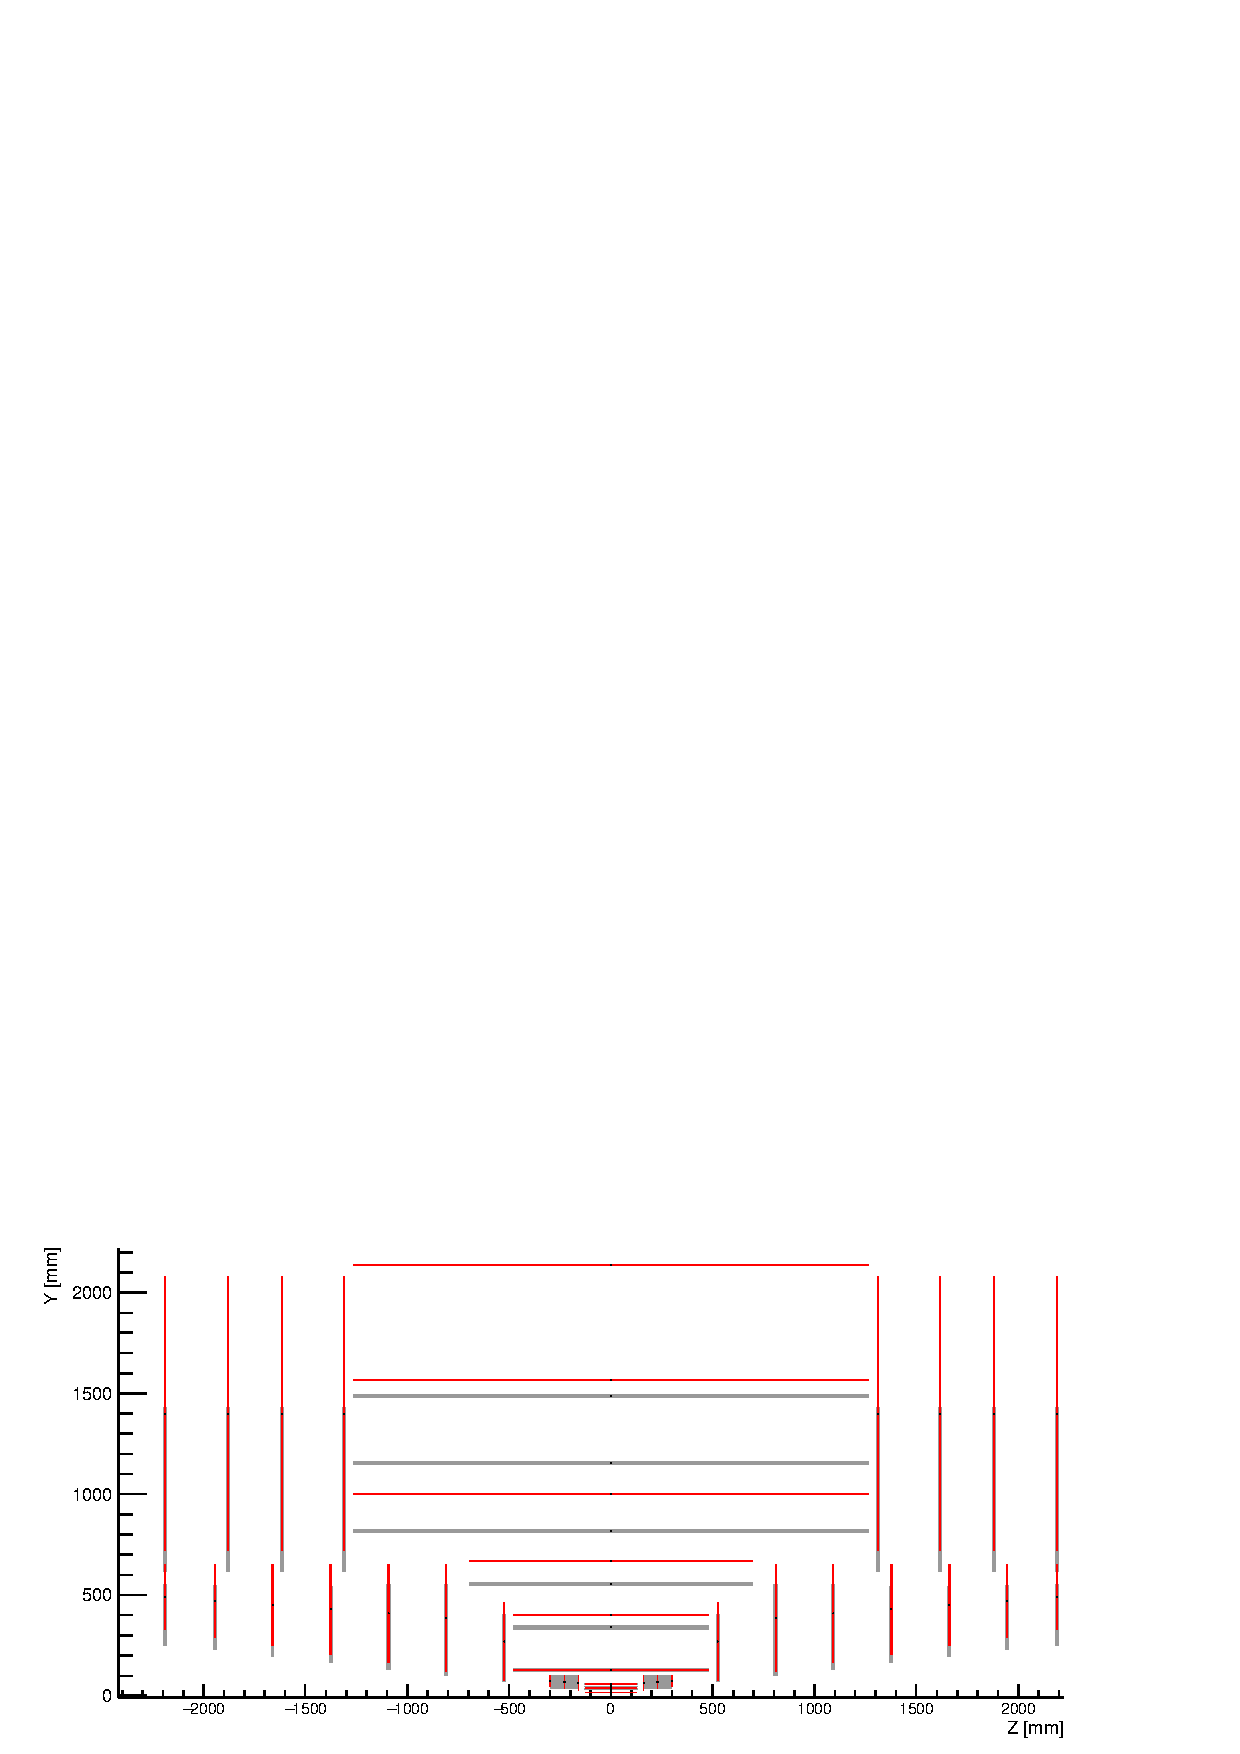
\includegraphics[width=12cm]{../geometryComparison_v3.pdf}};

%% HELPER draw advanced helping grid with axises:
% \draw(-0.5,-4) to[grid with coordinates] (11.5,4);
\end{tikzpicture}

  
\end{frame}
%*****************************************************************************


% %*****************************************************************************
% \begin{frame}{\large \large TODO Single particle ID efficiency}
% % TODO change legend for electron plot. ``Nominal'' -> ``Default Pandora''
% 
% \renewcommand{\yRefPosOne}{0}
% \renewcommand{\xRefPosOne}{5.3}
% \renewcommand{\xRefIncrementOne}{5.5}
% \begin{tikzpicture}[overlay]
% 
%  \node[inner sep=0pt] (tmp) at (\xRefPosOne-3,\yRefPosOne+1.5)
%     {\includegraphics[width=6cm]{../oct11_2017/test.pdf}};
% 
%  \node[inner sep=0pt] (tmp) at (\xRefPosOne+3,\yRefPosOne+1.5)
%     {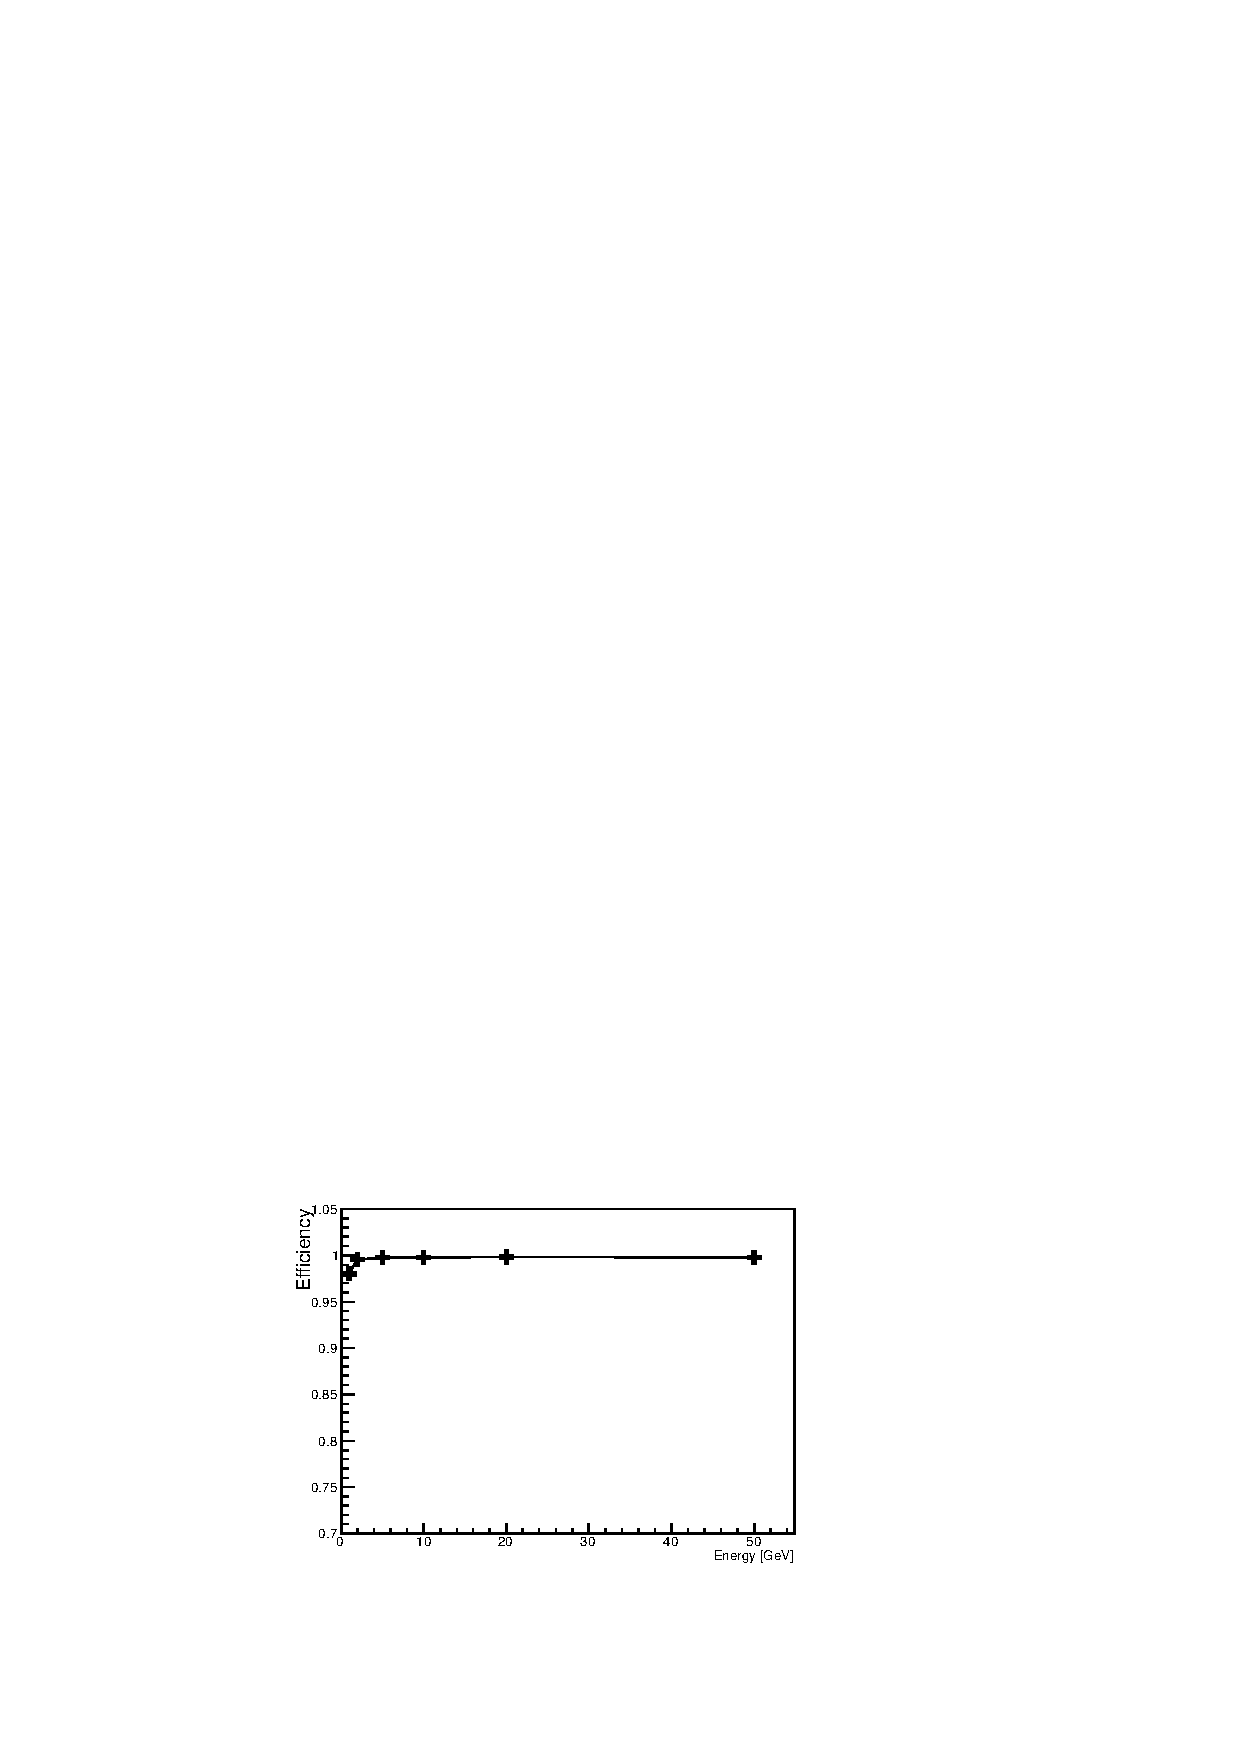
\includegraphics[width=6cm]{sep27/gamma_eff.pdf}};
% 
%  \node[inner sep=0pt] (tmp) at (\xRefPosOne-3,\yRefPosOne-2.7)
%     {\includegraphics[width=6cm]{sep27/pion_eff.pdf}};
% 
% %  \node[inner sep=0pt] (tmp) at (\xRefPosOne+3,\yRefPosOne-2.7)
% %     {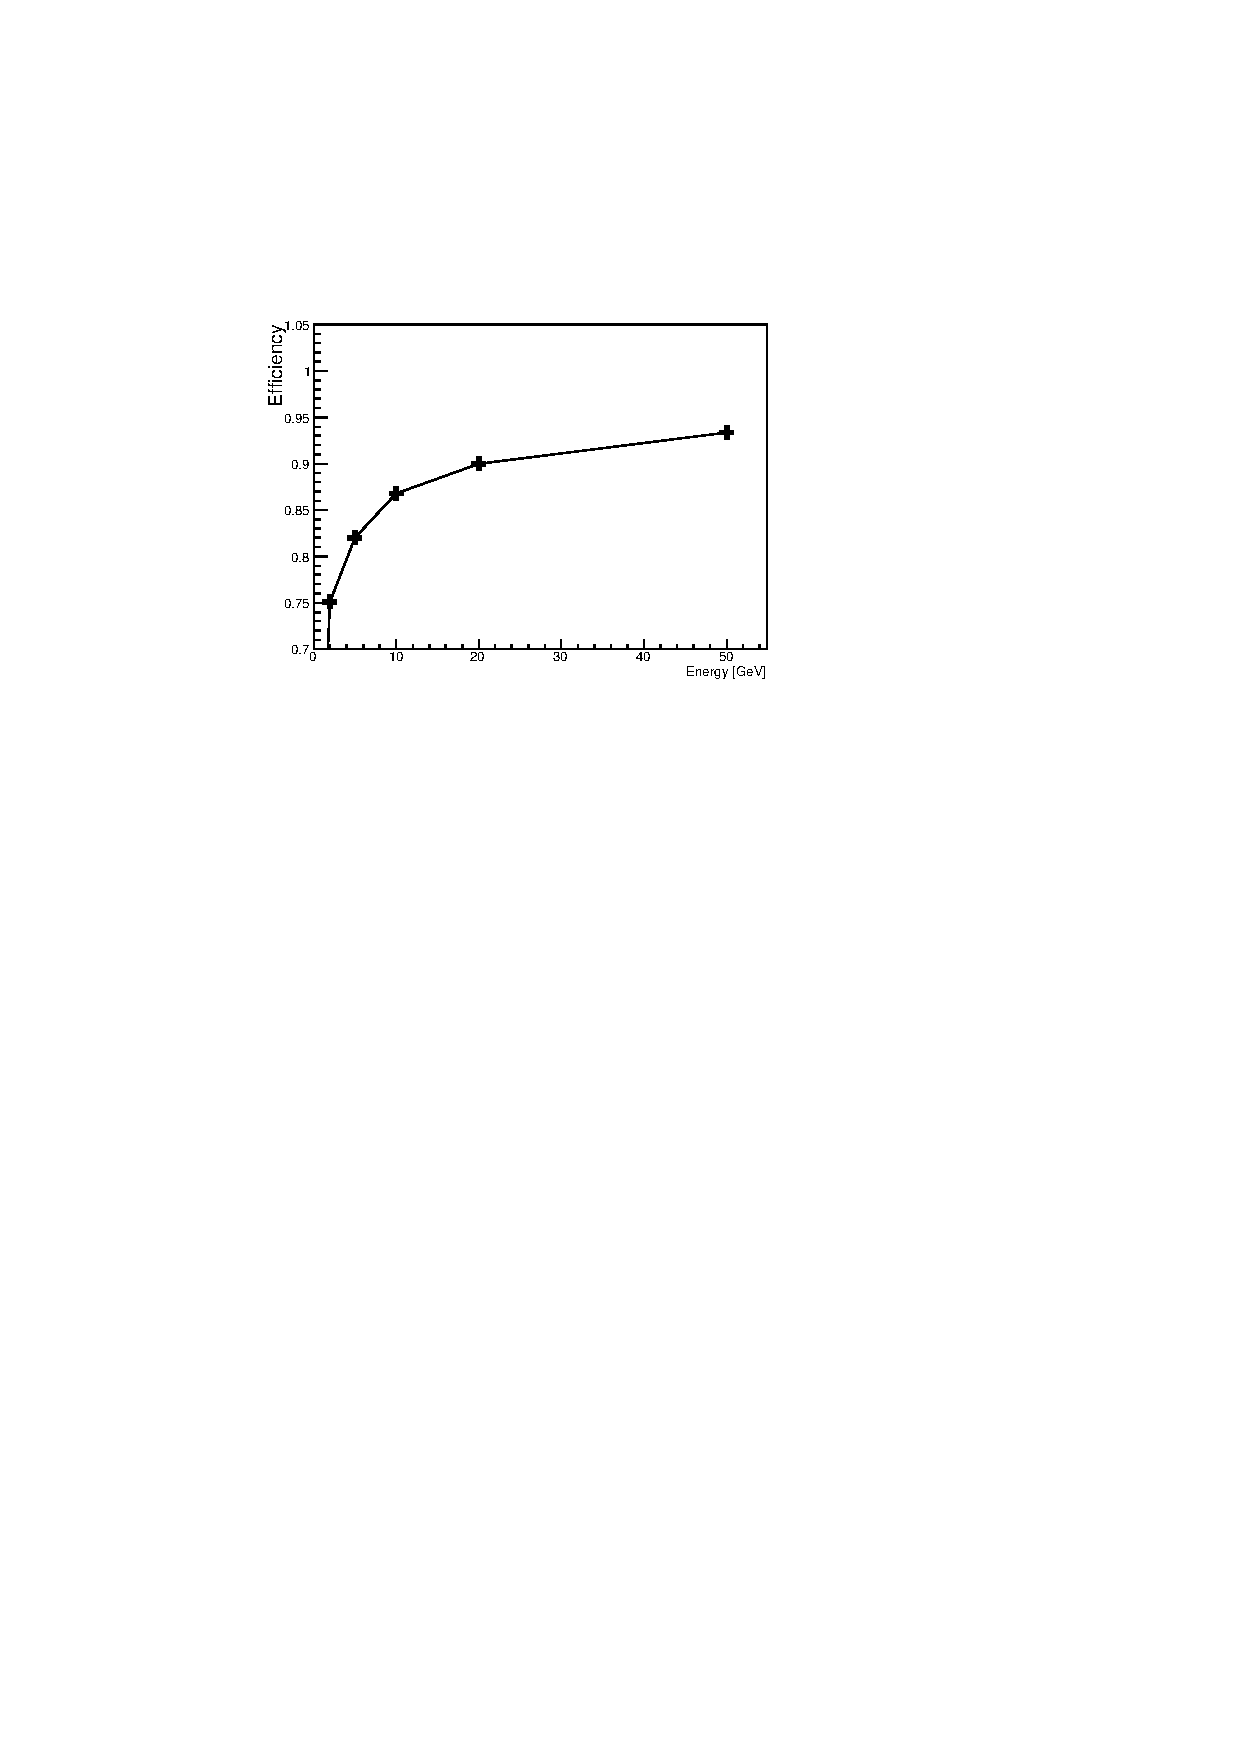
\includegraphics[width=6cm]{sep27/electron_eff.pdf}};
% 
% \node [Box] at (\xRefPosOne-3,\yRefPosOne+3.5) (box){%
% \myCenterBox{Electron}
% };
% 
% \node [Box] at (\xRefPosOne+3,\yRefPosOne+3.5) (box){%
% \myCenterBox{Photon}
% };
% 
% \node [Box] at (\xRefPosOne-3,\yRefPosOne-0.7) (box){%
% \myCenterBox{Pion}
% };
% 
% \node [Box] at (\xRefPosOne+3,\yRefPosOne-0.7) (box){%
% \myCenterBox{Muon}
% };
% 
% % \node [Box] at (\xRefPosOne,\yRefPosOne-4.65) (box){%
% %     \begin{minipage}{0.99\textwidth}
% % 
% %   \begin{itemize}
% %   \item ???
% %  \end{itemize}
% % 
% %     \end{minipage}
% % };
% 
% %% HELPER draw advanced helping grid with axises:
% % \draw(-0.5,-4) to[grid with coordinates] (11.5,4);
% \end{tikzpicture}
%  
% \end{frame}
% %*****************************************************************************
%*****************************************************************************
\begin{frame}{\large \large Neutral Particles Energy Resolution}
\renewcommand{\yRefPosOne}{0}
\renewcommand{\xRefPosOne}{5.3}
\renewcommand{\xRefIncrementOne}{5.5}
\begin{tikzpicture}[overlay]
 
 \node[inner sep=0pt] (tmp) at (\xRefPosOne-3,\yRefPosOne+0.7)
  {\includegraphics[width=6cm]{gammaRes_vs_energy.pdf}};

 \node[inner sep=0pt] (tmp) at (\xRefPosOne+3,\yRefPosOne+0.7)
  {\includegraphics[width=6cm]{kaon0LRes_vs_energy.pdf}};

 \node[inner sep=0pt] (tmp) at (\xRefPosOne-2.3,\yRefPosOne+2.65)
  {\tiny WORK IN PROGRESS};
 \node[inner sep=0pt] (tmp) at (\xRefPosOne+3.7,\yRefPosOne+2.65)
  {\tiny WORK IN PROGRESS};
  
\node [PixelBox] at (\xRefPosOne-3,\yRefPosOne-2.9) (box){
    \begin{minipage}{0.34\textwidth}
    \hspace{0.9cm}$\sigma_{E}/ E \simeq$ 1.6 $\%$  
    \\ reached for 100 GeV photons
    \end{minipage}
};

\node [PixelBox] at (\xRefPosOne+3,\yRefPosOne-2.9) (box){
    \begin{minipage}{0.34\textwidth}
    \hspace{0.9cm}$\sigma_{E}/ E \simeq$ 7.3 $\%$  
    \\ reached for 100 GeV K$_L^0$
    \end{minipage}
};

\node [Box] at (\xRefPosOne-3,\yRefPosOne+3.2) (box){%
  \myCenterBox{Photons, 60$^o<\theta<$120$^o$}
};

\node [Box] at (\xRefPosOne+3,\yRefPosOne+3.2) (box){%
  \myCenterBox{K$_L^0$, 60$^o<\theta<$120$^o$}
};

\node [Box] at (\xRefPosOne,\yRefPosOne-4) (box){%
    \begin{minipage}{0.99\textwidth}

  \begin{itemize}
  \item Good energy resolution for neutral particles
  \item Energy of charged particles is estimated from tracking
 \end{itemize}

    \end{minipage}
};
  
\end{tikzpicture}
\end{frame}
%*****************************************************************************



%*****************************************************************************
\begin{frame}{\large \large Jet Energy Resolution}
\renewcommand{\yRefPosOne}{-0.5}
\renewcommand{\xRefPosOne}{4.2}
\renewcommand{\xRefIncrementOne}{7.5}
\begin{tikzpicture}[overlay]

 \node[inner sep=0pt] (tmp) at (\xRefPosOne-1.7,\yRefPosOne+0.9)
  {\includegraphics[width=6cm]{../oct11_2017/jet_energy_res.pdf}};
  
 \node[inner sep=0pt] (tmp) at (\xRefPosOne+4.5,\yRefPosOne+0.9)
  {\includegraphics[width=6cm]{../oct11_2017/jet_energy.pdf}};

 \node[inner sep=0pt] (tmp) at (\xRefPosOne-1,\yRefPosOne+1.5)
  {\tiny WORK IN PROGRESS};
 \node[inner sep=0pt] (tmp) at (\xRefPosOne+5.4,\yRefPosOne+1.5)
  {\tiny WORK IN PROGRESS};
  
 \node[inner sep=0pt] (tmp) at (\xRefPosOne+4.5,\yRefPosOne-2.8)
  {\includegraphics[width=4cm]{../oct11_2017/jetRes_formula.png}
  };
 
  \node[inner sep=0pt] (tmp) at (\xRefPosOne+4.5,\yRefPosOne-3.5)
  {\myCenterBox[yellow]{\href{http://arxiv.org/abs/1209.4039}{arXiv:1209.4039}}  };
 
 
 
 
 
  \node [Box] at (\xRefPosOne-0.3,\yRefPosOne-2.8) (box){%
    \begin{minipage}{0.8\textwidth}
      \begin{itemize}
	\item Total energy is reconstructed with 1$\%$ accuracy:
	\begin{itemize}
	 \item 91 GeV: \hspace{0.07cm} 90.4 GeV
	 \item 380 GeV: 376.4 GeV
	\end{itemize}
	\item Jet energy resolution in barrel region:
	\begin{itemize}
	 \item 91 GeV: \hspace{0.07cm} 4.4 $\%$
	 \item 380 GeV: 3.5 $\%$ \\ [0.2cm]
	\end{itemize}
	\item comparable resolution with the CLIC detector 

      \end{itemize}
    \end{minipage}
  };
  
\end{tikzpicture}
\end{frame}
%*****************************************************************************



%*****************************************************************************
\begin{frame}{\large \large Summary}
 
 \renewcommand{\yRefPosOne}{0}
\renewcommand{\xRefPosOne}{5.3}
\renewcommand{\xRefIncrementOne}{5.5}
\begin{tikzpicture}[overlay]

      
\node [Box] at (\xRefPosOne,\yRefPosOne) (box){%
  \begin{minipage}{0.99\textwidth}
 \begin{itemize}
  \item The design of CLIC-inspired all-silicon detector for FCC-ee has been presented\\[0.6cm]
  \item Background studies demonstrate that dominant contribution to the detector occupancy originates 
  from $\gamma\gamma \to e^+e^-$ which constrains electronics readout time to $\approx$0.4 $\mu s$ 
  for VTX and Tracker detectors at 91.2 GeV. \\At 365 GeV it is much more relaxed because of the much larger bunch spacing 
  (8533 ns vs. 20 ns) \\[0.6cm]
  \item Performance studies based on the full simulation demonstrate that proposed detector design for FCC-ee provides
  comparable tracking and calorimetry performance w.r.t. CLIC detector \\[0.6cm]
%   \item The second detector design which consist of drift chamber and dual readout calorimeter 
  

%   \item Performance study based on the full simulation demonstrated impressive detector performance 
%   \item TODO to mention IDEA detector concept???
  
    \end{itemize}
  \end{minipage}
};
% \node[fancytitle, right=15pt] at (box.north west) {Transition Radiation Tracker};


% \node [PixelBox] at (\xRefPosOne,\yRefPosOne-2) (box){%
%   \begin{minipage}{0.99\textwidth}
%  \begin{itemize}
%      \item Something about IDEA detector concept???
%     \end{itemize}
%   \end{minipage}
% };

% \node [Box] at (\xRefPosOne-4.2,\yRefPosOne+0.4) (box){%
% \myCenterBox[PixelColor]{Next steps}
% };

% \node[fancytitle, right=15pt] at (box.north west) {Next steps};
% \node[fancytitle, right=15pt] at (box.north west) {LUCID};

\node[right] (textNode) at (3,-3) {
      { \large \bf Thank you for attention! }
    };

\end{tikzpicture}
  
\end{frame}
%*****************************************************************************

\backupbegin

%------------------------------------------------
\begin{frame}
\frametitle{BACKUP} 
 
\end{frame}
%------------------------------------------------

%*****************************************************************************
\begin{frame}{\large \large Coverage of VTX and Tracker detectors}
 
 
\renewcommand{\yRefPosOne}{0}
\renewcommand{\xRefPosOne}{5.3}
\renewcommand{\xRefIncrementOne}{5.5}
\begin{tikzpicture}[overlay]

%  \node[inner sep=0pt] (tmp) at (\xRefPosOne,\yRefPosOne-2.5)
%     {\includegraphics[width=12cm]{CLIC_vs_FCCee_trackingSystem.png}};


 \node[inner sep=0pt] (tmp) at (\xRefPosOne,\yRefPosOne-0.3)
    {\includegraphics[width=11cm]{../FCCee_tracking_coverage_july19.png}};

%     geometryComparison.png
% \node [Box] at (\xRefPosOne+2.5,\yRefPosOne+2) (box){%
%     \begin{minipage}{0.65\textwidth}
% 
%       \begin{itemize}
%         \item The same structure of the Inner and Outer trackers with larger dimentions.
% 	\item Similar coverage of the VTX + Tracker 
%       \end{itemize}
% 
%     \end{minipage}
% };
% \node[fancytitle, right=15pt] at (box.north west) {Transition Radiation Tracker};

\node [Box] at (\xRefPosOne,\yRefPosOne-4.3) (box){%
    \begin{minipage}{0.99\textwidth}

      \begin{itemize}
	\item Tracker coverage (number of sensitive layers as seen from IP). 
	\item More than 12 hits over theta range 8.6$^{\circ}$ - 171.4$^{\circ}$
      \end{itemize}

    \end{minipage}
};

\node [Box] at (\xRefPosOne+2.4,\yRefPosOne+2.5) (box){%
\myCenterBox{FCC-ee}
};

\node [Box] at (\xRefPosOne-2.4,\yRefPosOne+2.5) (box){%
\myVerySmallCenterBox{GEANTINOs}
};

%% HELPER draw advanced helping grid with axises:
% \draw(-0.5,-4) to[grid with coordinates] (11.5,4);
\end{tikzpicture}



 
\end{frame}
%*****************************************************************************


% %*****************************************************************************
% \begin{frame}{\large \large Luminosity monitor [TODO]}
%  
%  
% \renewcommand{\yRefPosOne}{0}
% \renewcommand{\xRefPosOne}{5.3}
% \renewcommand{\xRefIncrementOne}{5.5}
% \begin{tikzpicture}[overlay]
% 
% 
% %% HELPER draw advanced helping grid with axises:
% % \draw(-0.5,-4) to[grid with coordinates] (11.5,4);
% \end{tikzpicture}
% 
% 
% 
%  
% \end{frame}
% %*****************************************************************************

%*****************************************************************************
\begin{frame}{\large \large FCC-ee detector}
 
\renewcommand{\yRefPosOne}{0}
\renewcommand{\xRefPosOne}{5.3}
\renewcommand{\xRefIncrementOne}{5.5}
\begin{tikzpicture}[overlay]


 \node[TRTBox] (tmp) at (\xRefPosOne,\yRefPosOne-0.5)
  { 
    \begin{minipage}{0.8\textwidth}

    \resizebox{\columnwidth}{!}{%
      \begin{tabular}{lccc}
	 & CLIC & & FCC-ee \\[0.18cm]
	VTX Barrel & 31-60 mm & $\Longrightarrow$ & 17-59 mm \\[0.18cm]
	VTX Endcap & Spirals & $\Longrightarrow$ & Disks \\[0.18cm]
	Tracker radius & 1486 mm & $\Longrightarrow$ & 2100 mm \\[0.18cm]
% 	ECAL thickness & 202 mm & $\Longrightarrow$ & 202 mm \\[0.18cm]
% 	HCAL thickness & 44 $\times$ 7.5 $\lambda_0$ & $\Longrightarrow$ & 44 $\times$ 5.5 $\lambda_0$ \\[0.18cm]
	ECAL thickness & 40 layers, 22 X$_0$ & $\Longrightarrow$ & 40 layers, 22 X$_0$ \\[0.18cm]
	HCAL thickness & 60 layers, 7.5 $\lambda_I$ & $\Longrightarrow$ & 44 layers, 5.5 $\lambda_I$ \\[0.18cm]
	Yoke thickness & 1989 mm & $\Longrightarrow$ & 1521 mm \\[0.18cm]
	MDI (forward region) &  & $\Longrightarrow$ & $<$ 150 mrad \\[0.4cm]
	Solenoid field & 4 Tesla & $\Longrightarrow$ & 2 Tesla \\
	
      \end{tabular}%
    }
    \end{minipage}
  };
  


\node [Box] at (\xRefPosOne,\yRefPosOne+2.6) (box){%
\myCenterBox[TRTColor]{Overall dimensions of CLIC and FCC-ee detectors}
};
  
\end{tikzpicture}
\end{frame}
%*****************************************************************************


\backupend

\end{document}

